%-----------------------------------------------------------------------------
%
%               Template for sigplanconf LaTeX Class
%
% Name:         sigplanconf-template.tex
%
% Purpose:      A template for sigplanconf.cls, which is a LaTeX 2e class
%               file for SIGPLAN conference proceedings.
%
% Guide:        Refer to "Author's Guide to the ACM SIGPLAN Class,"
%               sigplanconf-guide.pdf
%
% Author:       Paul C. Anagnostopoulos
%               Windfall Software
%               978 371-2316
%               paul@windfall.com
%
% Created:      15 February 2005
%
%-----------------------------------------------------------------------------


\documentclass[preprint,10pt]{sigplanconf}

% The following \documentclass options may be useful:
%
% 10pt          To set in 10-point type instead of 9-point.
% 11pt          To set in 11-point type instead of 9-point.
% authoryear    To obtain author/year citation style instead of numeric.

\usepackage{amsmath}
% \usepackage{color}
\usepackage{listings,xspace}
\usepackage{amsthm}
\usepackage{mdframed}
\usepackage{xcolor}
\usepackage{fontspec}
\usepackage{graphicx}
\usepackage{setspace}
\usepackage{booktabs}
\usepackage{wasysym}
\usepackage{amsthm}
\usepackage{url}

\usepackage{caption}
\usepackage{subcaption}

\usepackage{bcprules}
\usepackage{prooftree}
\usepackage{multicol}

\lstdefinelanguage{Scala}%
{morekeywords={abstract,case,catch,char,class,%
    def,else,extends,final,%
    if,import,%
    match,module,new,null,object,override,package,private,protected,%
    public,return,super,this,throw,trait,try,type,val,var,with,implicit,%
  },%
  sensitive,%
  morecomment=[l]//,%
  morecomment=[s]{/*}{*/},%
  morestring=[b]",%
  morestring=[b]',%
  showstringspaces=false%
}[keywords,comments,strings]%

\lstset{language=Scala,%
  mathescape=true,%
  columns=[c]fixed,%
  basewidth={0.5em, 0.40em},%
  basicstyle=\tt,%
  xleftmargin=0.0cm
}

\makeatletter
\def \@ivtitleauthors#1#2#3#4{%
  \if \@andp{\@emptyargp{#2}}{\@emptyargp{#3}}%
    \noindent \@setauthor{40pc}{#1}{\@false}\par
  \else\if \@emptyargp{#3}%
    \noindent \@setauthor{17pc}{#1}{\@false}\hspace{3pc}%
              \@setauthor{17pc}{#2}{\@false}\par
  \else\if \@emptyargp{#4}%
    \noindent \@setauthor{17pc}{#1}{\@false}\hspace{3pc}%
              \@setauthor{17pc}{#3}{\@false}\par
  \else
    \noindent \@setauthor{9.3333pc}{#1}{\@false}\hspace{1.5pc}%
              \@setauthor{9.3333pc}{#2}{\@false}\hspace{1.5pc}%
              \@setauthor{9.3333pc}{#3}{\@false}\hspace{1.5pc}%
              \@setauthor{9.3333pc}{#4}{\@true}\par
    \relax
  \fi\fi\fi
  \vspace{20pt}}
\def \@maketitle {%
  \begin{center}
  \@settitlebanner
  \let \thanks = \titlenote
  {\leftskip = 0pt plus 0.25\linewidth
   \rightskip = 0pt plus 0.25 \linewidth
   \parfillskip = 0pt
   \spaceskip = .7em
   \noindent \LARGE \bfseries \@titletext \par}
  \vskip 6pt
  \noindent \Large \@subtitletext \par
  \vskip 12pt
  \ifcase \@authorcount
    \@latex@error{No authors were specified for this paper}{}\or
    \@titleauthors{i}{}{}\or
    \@titleauthors{i}{ii}{}\or
    \@titleauthors{i}{ii}{iii}\or
    \@ivtitleauthors{i}{ii}{iii}{iv}\or
    \@titleauthors{i}{ii}{iii}\@titleauthors{iv}{v}{}\or
    \@titleauthors{i}{ii}{iii}\@titleauthors{iv}{v}{vi}\or
    \@titleauthors{i}{ii}{iii}\@titleauthors{iv}{v}{vi}%
                  \@titleauthors{vii}{}{}\or
    \@titleauthors{i}{ii}{iii}\@titleauthors{iv}{v}{vi}%
                  \@titleauthors{vii}{viii}{}\or
    \@titleauthors{i}{ii}{iii}\@titleauthors{iv}{v}{vi}%
                  \@titleauthors{vii}{viii}{ix}\or
    \@titleauthors{i}{ii}{iii}\@titleauthors{iv}{v}{vi}%
                  \@titleauthors{vii}{viii}{ix}\@titleauthors{x}{}{}\or
    \@titleauthors{i}{ii}{iii}\@titleauthors{iv}{v}{vi}%
                  \@titleauthors{vii}{viii}{ix}\@titleauthors{x}{xi}{}\or
    \@titleauthors{i}{ii}{iii}\@titleauthors{iv}{v}{vi}%
                  \@titleauthors{vii}{viii}{ix}\@titleauthors{x}{xi}{xii}%
  \else
    \@latex@error{Cannot handle more than 12 authors}{}%
  \fi
  \vspace{1.75pc}
  \end{center}}
\makeatother

\theoremstyle{definition}
\newmdtheoremenv[hidealllines=true,topline=true,bottomline=true,skipabove=\baselineskip,skipbelow=\baselineskip]{defn}{Definition}[section]

\theoremstyle{definition}
\newmdtheoremenv[hidealllines=true,topline=true,bottomline=true,skipabove=\baselineskip,skipbelow=\baselineskip]{prop}{Property}[section]

% \theoremstyle{nonumberplain}
% \theoremstyle{definition}
% \newmdtheoremenv*[hidealllines=true,topline=true,bottomline=true,skipabove=\baselineskip,skipbelow=\baselineskip]{defnn}{Definition}[section]
\newtheorem*{defn*}{Definition}

% \newtheorem{defn}{Definition}[section]
% \newenvironment{defn}
  % {\begin{mdframed}[style=warning]\begin{mdef}}
  % {\end{mdef}\end{mdframed}}

% comments and notes
\newcommand{\comment}[1]{}
\newcommand{\note}[1]{{\bf $\clubsuit$ #1 $\spadesuit$}}
\newcommand{\ifreport}[1]{#1}
%\newcommand{\ifreport}[1]{}

\newcommand{\todo}{{\bf \colorbox{red}{\color{white}TODO:}}}
\newcommand{\ie}{{\em i.e.,~}}
\newcommand{\eg}{{\em e.g.,~}}
\newcommand{\term}[1]{\mbox{\texttt{#1}}}
\newcommand{\itl}[1]{\mbox{\textit{#1}}}

% commas and semicolons
\newcommand{\comma}{,\,}
\newcommand{\commadots}{\comma \ldots \comma}
\newcommand{\semi}{;\mbox{;};}
\newcommand{\semidots}{\semi \ldots \semi}

% spacing
\newcommand{\gap}{\quad\quad}
\newcommand{\biggap}{\quad\quad\quad}
\newcommand{\nextline}{\\ \\}
\newcommand{\htabwidth}{0.5cm}
\newcommand{\tabwidth}{1cm}
\newcommand{\htab}{\hspace{\htabwidth}}
\newcommand{\tab}{\hspace{\tabwidth}}
\newcommand{\linesep}{\ \hrulefill \ \smallskip}

\newcommand{\sectionline}{%
  \nointerlineskip \vspace{\baselineskip}%
  \hspace{\fill}\rule{0.5\linewidth}{.7pt}\hspace{\fill}%
  \par\nointerlineskip \vspace{\baselineskip}
}

% figures
\newcommand{\figurebox}[1]
        {\fbox{\begin{minipage}{\textwidth} #1 \medskip\end{minipage}}}
\newcommand{\twofig}[3]
        {\begin{figure*}[t]#3\ \hrulefill\
        \caption{\label{#1}#2}\end{figure*}}
\newcommand{\boxfig}[3]
        {\begin{figure*}\figurebox{#3\caption{\label{#1}#2}}\end{figure*}}
\newcommand{\figref}[1]
        {Figure~\ref{#1}}

% arrays
\newcommand{\ba}{\begin{array}}
\newcommand{\ea}{\end{array}}
\newcommand{\bda}{\[\ba}
\newcommand{\eda}{\ea\]}
\newcommand{\ei}{\end{array}}
\newcommand{\bcases}{\left\{\begin{array}{ll}}
\newcommand{\ecases}{\end{array}\right.}

%%%%%%%%%%%%%%%%%%%%%%%%%%%%%%%%%%%%%%%
%   Language abstraction commands     %
%%%%%%%%%%%%%%%%%%%%%%%%%%%%%%%%%%%%%%%

%% Relations
% Subtype
\newcommand{\sub}{<:}
% Type assignment
\newcommand{\typ}{:}
% reduction
\newcommand{\reduces}{\;\rightarrow\;}
% well-formedness
\newcommand{\wf}{\;\mbox{\textbf{wf}}}

%% Operators
% Type selection
\newcommand{\tsel}{\#}
% Function type
\newcommand{\tfun}{\rightarrow}
\newcommand{\dfun}[3]{(#1\!:\!#2) \Rightarrow #3}
% Conjunction
\newcommand{\tand}{\wedge}
% Disjunction
\newcommand{\tor}{\vee}
% Singleton type suffix
\newcommand{\sing}{.\textbf{type}}

%% Syntax
% Header for typing rules
\newcommand{\judgement}[2]{{\bf #1} \hfill \fbox{#2}}
% Refinement
\newcommand{\refine}[2]{\left\{#1 \Rightarrow #2 \right\}}
% Field definitions
\newcommand{\ldefs}[1]{\left\{#1\right\}}
% Member sequences
\newcommand{\seq}[1]{\overline{#1}}
% Lambda
\newcommand{\dabs}[3]{(#1\!:\!#2)\Rightarrow #3}
\newcommand{\abs}[3]{\lambda #1\!:\!#2.#3}
% Application
\newcommand{\app}[2]{#1\;#2}
% Substitution
\newcommand{\subst}[3]{[#1/#2]#3}
% Object creation
\newcommand{\new}[3]{\textbf{val }#1 = \textbf{new }#2 ;\; #3}
%\renewcommand{\new}[3]{#1 \leftarrow #2 \,\textbf{in}\, #3}
% Field declaration
\newcommand{\Ldecl}[3]{#1 \typ #2..#3}%{#1 \operatorname{>:} #2 \operatorname{<:} #3}
\newcommand{\ldecl}[2]{#1 \typ #2}
% Top and Bottom
\newcommand{\Top}{\top}%{\textbf{Top}}
\newcommand{\Bot}{\bot}%\textbf{Bot}}
% Environment extension
\newcommand{\envplus}[1]{\uplus \{ #1 \}}

\newcommand{\reduction}[4]{#1, #2 \reduces #3, #4}
\newcommand{\reducebig}[6]{#1, #2, #3 \;\Downarrow\; #4, #5, #6}
\newcommand{\evaluate}[5]{#1, #2, #3 \;\Downarrow\; #4, #5}
\newcommand{\evalcap}[8]{#1, #2, #3, #4 \;\Downarrow\; #5, #6, #7, #8}
\newcommand{\evalcapbreak}[8]{#1, #2, #3, #4 \;\Downarrow\; \\ #5, #6, #7, #8}
\newcommand{\evalcapfin}[9]{#2, #3, #4, #5 \;\Downarrow_{#1}\; #6, #7, #8, #9}

\newcommand{\sframe}[3]{\langle #1, #2, #3 \rangle}
\newcommand{\stack}[4]{#1 \sframe {#2} {#3} {#4}}
\newcommand{\reduce}[4]{#1, #2 \;\longrightarrow\; #3, #4}
\newcommand{\reducebreak}[4]{#1, #2 \\ \;\longrightarrow\; #3, #4}

\newcommand{\sreduce}[6]{#1, #2, #3 \;\longrightarrow\; #4, #5, #6}
\newcommand{\sreducebreak}[6]{#1, #2, #3 \\ \;\longrightarrow\; #4, #5, #6}
\newcommand{\sreducestar}[6]{#1, #2, #3 \;\longrightarrow^{\ast}\; #4, #5, #6}

% misc identifiers
\newcommand{\dom}{\mbox{\sl dom}}
\newcommand{\fn}{\mbox{\sl fn}}
\newcommand{\bn}{\mbox{\sl bn}}
\newcommand{\sig}{\mbox{\sl sig}}
\newcommand{\IF}{\mbox{\mathem if}}
\newcommand{\OTHERWISE}{\mbox{\mathem otherwise}}
\newcommand{\strongexpand}{\prec\!\!\prec}
\newcommand{\weakexpand}{\prec}
\newcommand{\spcomma}{~,~}

\begin{document}

\setmainfont[Mapping=tex-text]{Times New Roman}
\setmonofont[Scale=0.8,BoldFont={Consolas Bold}]{Consolas}

\conferenceinfo{OOPSLA '13}{October 26-31, Indianapolis, IN, USA.}
\copyrightyear{2013}
\copyrightdata{[to be supplied]}

% \titlebanner{banner above paper title}        % These are ignored unless
% \preprintfooter{short description of paper}   % 'preprint' option specified.

\title{Object-Oriented Pickler Combinators}
\subtitle{and an Extensible Generation Framework}

\authorinfo{Heather Miller}
           {EPFL, Switzerland}
           {heather.miller@epfl.ch}
\authorinfo{Philipp Haller}
           {Typesafe, Inc.}
           {philipp.haller@typesafe.com}
\authorinfo{Eugene Burmako}
           {EPFL, Switzerland}
           {eugene.burmako@epfl.ch}
\authorinfo{Martin Odersky}
           {EPFL, Switzerland}
           {martin.odersky@epfl.ch}

\maketitle

\begin{abstract}

Serialization or pickling, i.e., persisting runtime objects by converting them
into a binary or text representation, is ubiquitous in distributed programming.
Pickler combinators are a popular approach from functional programming designed to
alleviate some of the tedium of writing pickling code by hand, but they don't
translate well to object-oriented programming due to qualities like open class
hierarchies and subtyping polymorphism. Furthermore, both functional pickler
combinators and Java-based serialization frameworks tend to be tied to a
specific pickle format, leaving programmers no choice of how their data is
persisted. In this paper, we present object-oriented pickler combinators and a
framework\footnote{\url{http://github.com/scala/pickling/}} for
generating them at compile-time, called \textit{scala/pickling}. While specifically
designed for the Scala programming language, many aspects of our
approach are applicable in other statically-typed object-oriented
languages. Our framework is
extensible: (1) using Scala's implicit parameters, users can add their own
easily interchangeable pickle format, (2) using the type class pattern, users can
provide their own custom picklers to override the default behavior of
the pickling framework. In addition to extensibility and need for little to
no boilerplate, the static generation of our OO picklers enables
significant performance improvements. In microbenchmarks, our framework
achieves a factor 6 speedup over Java Serialization, and performs on
par or up to 3 times faster than popular fast Java serialization frameworks like Kryo.

% \todo mention Akka \& Spark?
% We go on to evaluate
% our framework on two large industrial-strength frameworks for distributed
% computing, Akka and Spark, and show improved performance and a reduction of
% lines of serialization-related code for both projects.

\end{abstract}

\category{D.3.2}{Programming Languages}{Language Classifications --
  multiparadigm languages, object-oriented languages, applicative
  (functional) languages}
\category{D.3.3}{Programming Languages}{Language Constructs and
  Features -- input/output}

% \terms
% term1, term2

\keywords
Serialization, pickling, meta-programming, distributed programming, Scala

\section{Introduction}

With the growing trend towards cloud computing and mobile applications,
distributed programming has entered the mainstream. As more and more
traditional applications migrate to the cloud, the demand for interoperability between
different services is at an all-time high, and is increasing. At the center of
it all is communication. Whether we consider a cluster of commodity machines
churning through a massive data-parallel job, or a smartphone interacting with
a social network, all are ``distributed'' jobs, and all share the need to
communicate in various ways, in many formats, even within the same
application.

A central aspect to this communication that has received surprisingly little
attention in the literature is the need to serialize, or {\em pickle} objects
{\em i.e.,} to persist in-memory data by converting them to a binary, text, or
some other representation. On the JVM, serialization has long been
acknowledged as having a high overhead \cite{Welsh2000, Carpenter1999}, with
some estimates purporting object serialization to account for 25-65\% of the
cost of remote method invocation, and which go on to observe that the cost of
serialization grows with growing object structures up to 50\%
\cite{Philippsen2000, Maassen1999}.

Due to the prohibitive cost of using Java Serialization in high-performance
distributed applications, many frameworks for distributed computing, like
Akka~\cite{Akka}, Spark~\cite{Zaharia2012}, SCADS \cite{Armbrust2009}, and
others, provide support for higher-performance alternative frameworks such as
Google's Protobuf~\cite{Protobuf}, Apache Avro~\cite{Avro}, or
Kryo~\cite{Kryo}. However, the higher efficiency typically comes at the cost
of weaker or no type safety, a fixed serialization format, more restrictions
placed on the objects to-be-serialized, or only rudimentary language
integration.

This paper takes a step towards more principled open programming through a new
foundation for pickling in object-oriented languages. We present object-oriented
picklers and \textit{scala/pickling}, a framework for their generation either at runtime or at
compile time. The introduced notion of object-oriented pickler combinators
extends pickler combinators known from functional
programming~\cite{Kennedy2004} with support for object-oriented concepts such
as subtyping, mix-in composition,  and object identity in the face of cyclic
object graphs. In contrast to pure functional-style
pickler combinators, we employ static, type-based meta programming to compose
picklers at compile time. The resulting picklers are efficient, since the
pickling code is generated statically as much as possible, avoiding the
overhead of runtime reflection~\cite{Gil2008,Dubochet2011}.

Furthermore, the presented pickling framework is extensible in several
important ways. First, building on an object-oriented type-class-like
mechanism~\cite{Oliveira2010}, our approach enables retroactively adding
pickling support to existing, unmodified types. Second, our framework provides
pluggable pickle formats which decouple type checking and pickler composition
from the lower-level aspects of data formatting. This means that the type
safety guarantees provided by type-specialized picklers are ``portable'' in
the sense that they carry over to different pickle formats.

The design of our framework has been guided by the following principles:
\begin{itemize}
\item {\bf Ease of use}. The programming interface aims to require as little
pickling boilerplate as possible. Thanks to dedicated support by the
underlying virtual machine, Java's serialization~\cite{JavaSerialization}
requires only little boilerplate, which mainstream Java developers have come
to expect. Our framework aims to be useable in production environments, and
must, therefore, be able to integrate with existing systems with minimal
changes.

\item {\bf Performance}. The generated picklers should be efficient enough  so
as to enable their use in high-performance distributed, ``big data'', and
cloud applications. One factor driving practitioners away from Java's default
serialization mechanism is its high runtime overhead compared to alternatives
such as Kryo, Google's protocol buffers or Apache's Avro serialization
framework. However, frameworks such as the latter offer only minimal language
integration.

\item {\bf Extensibility}. It should be possible to add pickling support to existing
types retroactively. This resolves a common issue in Java-style serialization
frameworks where classes have to be marked as serializable upfront,
complicating unanticipated change. Furthermore, type-class-like extensibility
enables pickling also for types provided by the underlying runtime environment
(including built-in types), or types of third-party libraries.

\item {\bf Pluggable Pickle Formats}. It should be possible to easily swap target
pickle formats, or for users to provide their own customized format. It is not
uncommon for a distributed application to require multiple formats for
exchanging data, for example an efficient binary format for exchanging system
messages, or JSON format for publishing feeds. Type-class-like extensibility
makes it possible for users to define their own pickle format, and to easily
{\em swap it in} at the use-site.

\item {\bf Type safety}. Picklers should be type safe through (a) type
specialization and (b) dynamic type checks when unpickling to transition
unpickled objects into the statically-typed ``world'' at a well-defined program
point.

\item {\bf Robust support for object-orientation}. Concepts such as subtyping
and mix-in composition are used very commonly to define
regular object types in object-oriented languages. Our approach is also general,
supporting object graphs with cycles. Since our framework does
without a separate data type description language ({\em e.g.,} a schema), it
is important that regular type definitions are sufficient to describe tahe
types to-be-pickled. The Liskov substitution principle is used as a guidance
surrounding the substitutability of both objects to-be-pickled and first-class
picklers.
\end{itemize}


\subsection{Selected Related Work}

Some OO languages like Java and runtime environments like the JVM or
.NET provide serialization for arbitrary types, provided entirely by
the underlying virtual machine. While this approach is very convenient
for the programmer there are also several issues: (a) the pickling
format cannot be exchanged (Java), (b) serialization relies on runtime
reflection which hits performance, and (c) existing classes that do
not extend a special marker interface are not serializable, which
often causes oversights resulting in software engineering costs. In
functional languages, pickler
combinators~\cite{Kennedy2004,Elsman2005} can reduce the effort of
manually writing pickling and unpickling functions to a large
extent. However, existing approaches do not support object-oriented
concepts such as subtyping polymorphism. Moreover, it is not clear
whether local type inference as required in OO languages would yield a
comparable degree of conciseness, acceptable to programmers used to
Java-style serialization.  Nonetheless, our approach builds on pickler
combinators, capitalizing on their powerful composability.

Our approach of retrofitting existing types with pickling support
builds on implicits in Scala~\cite{Oliveira2010} and is reminiscent of
other type-class-like mechanisms, such as JavaGI~\cite{WehrT11} or C++
Concepts~\cite{ReisS06}.

Additionally, in an effort to further reduce the boilerplate required
to define or compose picklers using existing picklers, we present a
framework for automatically generating picklers for compound types
based on picklers for their component types. Given the close
relationship of our implicit picklers to type classes, this generation
mechanism is related to Haskell's {\em deriving}
mechanism~\cite{MagalhaesDJL10}. One of the main differences is that
our mechanism is faithful to subtyping. So far, our mechanism is
specialized for pickling; an extension to a generic mechanism for
composing type class instances is left for future work.

We discuss other related work in Section \ref{sec:related-work}.

\subsection{Contributions}

This paper makes the following contributions:

\begin{itemize}

\item An extension to pickler combinators, well-known in functional
programming, to support the core concepts of object-oriented programming,
namely subtyping polymorphism, open class hierarchies, and object identity.

\item A framework based on object-oriented pickler combinators which (a)
enables retrofitting existing types with pickling support, (b) supports
automatically generating picklers at compile time and at runtime, (c) supports
pluggable pickle formats, and (d) does not require changes to the host
language or the underlying virtual machine.

\item A complete implementation of the presented approach in and for Scala
\footnote{See \url{http://github.com/scala/pickling/}}.

\item An experimental evaluation comparing the performance of our framework
with Java serialization and Kryo.

\end{itemize}


% \subsection{Reflection}
% \label{sec:reflection}




% \paragraph{Macro Annotations.} Unlike macro defs, macro annotations are capable
% of {\em adding members} to classes which carry their annotation.

% \begin{lstlisting}
% @withNewToString
% class D { ... }
% \end{lstlisting}

% The \verb|withNewToString| annotation is defined using a standard class
% definition by extending a special \verb|MacroAnnotation| marker trait, and by
% implementing a special \verb|transform| method as a macro:

% \begin{lstlisting}
% class withNewToString extends MacroAnnotation {
%   def transform = macro transform_impl
%   def transform_impl = { ... }
% }
% \end{lstlisting}

% The \verb|transform| macro implementation is passed the AST of the annotated class
% definition (the AST of ``\verb|class D { ... }|''), and returns a possibly changed AST
% as the new class definition (which could have added members, changed
% constructor parameters etc.)

\section{Overview and Usage}
\label{sec:overview}

\subsection{Basic Usage}

Scala/pickling was designed so as to require as little
boilerplate from the programmer as possible. For that reason, pickling or
unpickling an object \term{obj} of type \term{Obj} requires simply,

\begin{lstlisting}
import scala.pickling._
val pickl = obj.pickle
val obj2 = pickl.unpickle[Obj]
\end{lstlisting}

Here, the \term{import} statement imports scala/pickling, the method
\term{pickle} triggers static pickler generation, and the method
\term{unpickle} triggers static unpickler generation, where \verb|unpickle| is
parameterized on \verb|obj|'s precise type \verb|Obj|. Note that not every
type has a \term{pickle} method; it is implemented as an extension method
using an {\em implicit conversion}. This implicit conversion is imported into
scope as a member of the \term{scala.pickling} package.

\paragraph{Implicit conversions.} Implicit conversions can be thought of as
methods which can be implicitly invoked based upon their type, and whether or
not they are present in implicit scope. Implicit conversions carry the
\term{implicit} keyword before their declaration. The \verb|pickle| method is
provided using the following implicit conversion (slightly simplified):

\begin{lstlisting}
implicit def PickleOps[T](picklee: T) =
  new PickleOps[T](picklee)

class PickleOps[T](picklee: T) {
  def pickle: Pickle = ...
  ...
}
\end{lstlisting}

In a nutshell, the above implicit conversion is implicitly invoked, passing
object \verb|obj| as an argument, whenever the \verb|pickle| method is invoked
on \verb|obj|. The above example can be written in a form where all
invocations of implicit methods are explicit, as follows:

\begin{lstlisting}
val pickl = PickleOps[Obj](obj).pickle
val obj2 = pickl.unpickle[Obj]
\end{lstlisting}


Optionally, a user can
import a \term{PickleFormat}. By default, our framework provides a
Scala Binary Format, an efficient representation based on arrays of bytes,
though the framework provides other formats which can easily be imported,
including a JSON format. Furthermore, users can easily extend the framework by
providing their own \term{PickleFormat}s (see Section \ref{sec:pickleformat}).

Typically, the framework generates the required pickler itself inline in the
compiled code, using the \term{PickleFormat} in scope. In the case of JSON,
for example, this amounts to the generation of string concatenation code and
field accessors for getting runtime values, all of which is inlined, resulting
in high performance (see Section~\ref{sec:evaluation}).

In rare cases, however, it is necessary to fall back to runtime picklers which
use runtime reflection to access the state that is being pickled and
unpickled. For example, a runtime pickler is used when pickling instances of a
generic subclass of the static class type to-be-pickled.

Using scala/pickling, it's
also possible to pickle and unpickle subtypes, even if the pickle and unpickle
methods are called using supertypes of the type to-be-pickled.
For example,

\begin{lstlisting}
class Person(val name: String)
class Firefighter(override val name: String, val since: Int)
  extends Person(name)

val ff = new Firefighter("Jim", 2005)
val pickl = ff.pickle[Person]
val ff2 = pickl.unpickle[Person]
\end{lstlisting}

In the above example, the runtime type of \term{ff2} will correctly be
\term{Firefighter}.

This perhaps raises an important concern-- what if the type that is passed as
a type argument to method \term{unpickle} is incorrect? In this case, the
framework will fail with a runtime exception at the call-site of
\term{unpickle}. This is an improvement over other frameworks, which have less
type information available at runtime, resulting in wrongly unpickled objects
often propagating to other areas of the program before an exception is thrown.

Scala/pickling is also able to unpickle values of static type
\term{Any}. Scala's pattern-matching syntax can make unpickling on less-specific
types quite convenient, for example:

\begin{lstlisting}
val unpickld = pickl.unpickle[Any] match {
  case Firefighter(name, since) => ...
  case x: Int => ...
  ...
}
\end{lstlisting}

Beyond dealing with subtypes, our pickling framework supports
pickling/unpickling most Scala types, including generics, case classes, and
singleton objects. Passing a type argument to pickle, whether inferred or
explicit, which is an unsupported type leads to a compile-time error. This
avoids a common problem in Java-style serialization where non-serializable
types are only discovered at runtime, in general. Function types, however, are
not yet supported, and are planned future work.

\subsection{Advanced Usage}
\label{sec:pickleable-annotation}

\paragraph{$@$pickleable Annotation.} To handle subtyping correctly, the
pickling framework generates dispatch code which delegates to a pickler
specialized for the runtime type of the object to-be-pickled, or, if the
runtime type is unknown, which is to be expected in the presence of separate
compilation, to a generic, but slower, runtime pickler.

For higher performance, the scala/pickling additionally provides an
annotation which at compile-time inserts a runtime type test to check whether
the runtime class extends a certain class/trait; in which case, we call the
method that returns the pickler specialized for that runtime class. If the
class/trait has been annotated, the returned pickler has been generated
statically (when the annotation, implemented using a macro, is expanded in
each subclass, transitively).

This \verb|@pickleable| annotation enables:

\begin{itemize}
\item library authors to guarantee to their clients that picklers for separately-compiled
subclasses are fully generated at compile-time;

\item faster picklers in general because one need not worry about having to
fallback on a runtime pickler.
\end{itemize}

For example, assume the following class \verb|Person| and its subclass
\verb|Firefighter| are defined in separately-compiled code.

\begin{lstlisting}
// Library code
@pickleable class Person(val name: String)

// Client code
class Firefighter(override val name: String, salary: Int)
  extends Person(name)
\end{lstlisting}

Note that class \verb|Person| is annotated with the \verb|@pickleable|
annotation. \verb|@pickleable| is a {\em macro annotation} which generates
additional methods for obtaining type-specialized picklers (and unpicklers).
With the \verb|@pickleable| annotation expanded, the code for class
\verb|Person| looks roughly as follows:

\begin{lstlisting}
class Person(val name: String)
    extends PickleableBase {
  def pickler: SPickler[_] =
    implicitly[SPickler[Person]]
  ...
}
\end{lstlisting}

First, note that the supertypes of \verb|Person| now additionally include the
trait \verb|PickleableBase|; it declares the abstract methods that the
expansion of the macro annotation ``fills in'' with concrete methods. In this
case a \verb|pickler| method is generated which returns an
\verb|SPickler[_]|.\footnote{The notation \texttt{SPickler[\_]} is short for
the existential type \texttt{SPickler[t] forSome \{ type t \}}. It is necessary
here, because picklers must be invariant in their type parameter, see
Section~\ref{sec:unanticipated}.} Note that the \verb|@pickleable| annotation
is defined in a way where pickler generation is triggered in both
\verb|Person| and its subclasses.

Here, we obtain an instance of \verb|SPickler[Person]| by means of implicits.
The \verb|implicitly| method, part of Scala's standard library, is defined as
follows:

\begin{lstlisting}
def implicitly[T](implicit e: T) = e
\end{lstlisting}
\noindent
Annotating the parameter (actually, the parameter list) using the
\verb|implicit| keyword means that in an invocation of \verb|implicitly|, the
implicit argument list may be omitted if, for each parameter of that list,
there is exactly one value of the right type in the {\em implicit scope}. The
implicit scope is an adaptation of the regular variable scope; imported
implicits, or implicits declared in an enclosing scope are contained in the
implicit scope of a method invocation.

As a result, \verb|implicitly[T]| returns the uniquely-defined implicit value
of type \verb|T| which is in scope at the invocation site. In the context of
picklers, there might not be an implicit value of type \verb|SPickler[Person]|
in scope (in fact, this is typically only the case with custom picklers). In
that case, a suitable pickler instance is generated using a macro def.

\paragraph{Macro defs.} Macro defs are methods that are transparently loaded
by the compiler and executed (or expanded) during compilation. A macro is
defined as if it is a normal method, but it is linked using the \verb|macro|
keyword to an additional method that operates on abstract syntax trees.

\begin{lstlisting}
def assert(x: Boolean, msg: String): Unit =
  macro assert_impl
def assert_impl(c: Context)
  (x: c.Expr[Boolean], msg: c.Expr[String]):
                            c.Expr[Unit] = ...
\end{lstlisting}

In the above example, the parameters of \verb|assert_impl| are syntax trees,
which the body of \verb|assert_impl| will operate on, itself returning an AST
of type \verb|Expr[Unit]|. It is \verb|assert_impl| that is expanded and
evaluated at compile-time. Its result is then inlined at the callsite of
\verb|assert| and the inlined result is typechecked It is also important to
note that implicit defs as described above can be implemented as macros.

Scala/pickling provides an implicit macro def returning picklers for arbitrary
types. Slightly simplified, it is declared as follows:

\begin{lstlisting}
implicit def genPickler[T]: SPickler[T]
\end{lstlisting}

This macro def is expanded when invoking \newline
\verb|implicitly[SPickler[T]]| if
there is no implicit value of type \verb|SPickler[T]| in scope.


\paragraph{Custom Picklers.} It is possible to use manually written picklers
in place of generated picklers. Typical motivations for doing so are (a)
improved performance through specialization and optimization hints, and (b) custom pre-pickling and post-unpickling
actions; such actions may be required to re-initialize an object
correctly after unpickling. Creating custom picklers is greatly facilitated by
modular composition using object-oriented pickler combinators. The design of
these first-class object-oriented picklers and pickler combinators is
discussed in detail in the following Section~\ref{sec:oopicklers}.


% \section{Background: Reflection in Scala}
% \label{sec:reflection}

% Reflection is the ability of a program to inspect, and possibly even modify
% itself at runtime. Before Scala 2.10, Scala did not have any reflection
% capabilities of its own. Instead, one could use Java reflection which provided
% basic but limited runtime reflection capabilities. In Scala 2.10, a new
% reflection library was introduced not only to address the shortcomings of
% Java's runtime reflection on Scala-specific and generic types, but to also add
% a more powerful toolbox of general reflective capabilities to Scala. Along
% with full-featured runtime reflection for Scala types and generics, Scala 2.10
% also ships with compile-time reflection capabilities, in the form of macros
% (covered in Section \ref{sec:macros}), as well as the ability to reify Scala
% expressions into abstract syntax trees (ASTs).

% \paragraph{TypeTags.} One aspect of runtime reflection that was introduced in
% Scala 2.10 is the notion of \verb|TypeTag|s. As with other JVM languages,
% Scala's types are erased at compile time. \verb|TypeTag|s can be thought of as
% objects which carry along all type information available at compile time, to
% runtime. As we will see, \verb|TypeTag|s will prove to be invaluable in
% situations where precise type information would otherwise not be available at runtime.

% \paragraph{Unified Runtime/Compile-time Reflection API.} Another important
% aspect of Scala's reflection library is the one-to-one correspondence between
% Scala Reflection's compile-time (\ie macros) and runtime APIs. Each API is
% parameterized on a so-called \verb|Universe|, an object which serves as the
% entry point to Scala reflection, and which provides all principal concepts
% used in reflection, such as \verb|Type|s, \verb|Tree|s, and
% \verb|Annotation|s. Depending on the task at hand, the choice between runtime
% and compile-time reflection is as easy as selecting either a compile-time or a
% runtime \verb|Universe|. As we will see, this enables maximum code
% reuse in that a fallback runtime pickler generation mechanism can be achieved
% by simply reusing the code for static generation, and parameterizing it on a
% runtime \verb|Universe|.


% \begin{figure*}[t]
% $\ba[t]{ll@{\hspace{2mm}}l@{\hspace{2mm}}l@{\hspace{2mm}}l}
% F ::= & [] ~|~ F[x \mapsto r]    & \mbox{envir.}~(x \notin dom(F))
%       & r \in RefLocs            & \mbox{reference location} \\
% H ::= & [] ~|~ H[r \mapsto o]    & \mbox{heap}
%       & o ::= (T, F)             & \mbox{object}
% \ea$
% \caption{Environments, objects, and heaps.}
% \label{fig:objects-heaps}
% \end{figure*}

\section{Object-Oriented Picklers}\label{sec:oopicklers}

In the first part of this section (\ref{sub:picklers-scala}) we introduce
picklers as first-class objects, and, using examples, motivate the contracts
that valid implementations must guarantee. We demonstrate that the introduced
picklers enable modular, object-oriented pickler combinators, \ie methods for
composing more complex picklers from simpler primitive picklers.

In the second part of this section (\ref{sub:picklers-formal}) we present a
formalization of object-oriented picklers based on an operational semantics.

\subsection{Picklers in Scala}\label{sub:picklers-scala}

In scala/pickling, a {\em static pickler} for some type \verb|T| is an
instance of trait \verb|SPickler[T]| which has a single abstract method
\verb|pickle|:

\begin{lstlisting}
    trait SPickler[T] {
      def pickle(obj: T, builder: PBuilder): Unit
    }
\end{lstlisting}
\noindent
For a concrete type, say, class \verb|Person| from Section~\ref{sec:overview},
the \verb|pickle| method of an \verb|SPickler[Person]| converts
\verb|Person| instances to a pickled format, using a {\em pickle builder} (the
\verb|builder| parameter). Given this definition, picklers ``are type safe in
the sense that a type-specialized pickler can be applied only to values of the
specialized type.''~\cite{Elsman2005}. The pickled result is not returned
directly; instead, it can be requested from the \verb|builder| using its
\verb|result()| method. Example:

\begin{lstlisting}
    val p = new Person("Jack")
    ...
    val personPickler   = implicitly[SPickler[Person]]
    val builder         = pickleFormat.createBuilder()
    personPickler.pickle(p, builder)
    val pickled: Pickle = builder.result()
\end{lstlisting}
\noindent
In the above example, invoking \verb|implicitly[SPickler[Person]]| either
returns a regular implicit value of type \verb|SPickler[Person]| that is in
scope, or, if it doesn't exist, triggers the (compile-time) generation of a
type-specialized pickler (see Section~\ref{sec:generation}). To use the
pickler it is also necessary to obtain a pickle builder. Since pickle formats
in scala/pickling are exchangable (see Section~\ref{sec:pickleformat}), pickle
builders depend on specific pickle formats, which provide builder factory
methods.

The \verb|pickled| result has type \verb|Pickle| which wraps a concrete
representation, such as a byte array (\eg for binary formats) or a string (\eg
for JSON). The abstract \verb|Pickle| trait is defined as follows:

\begin{lstlisting}
trait Pickle {
  type ValueType
  type PickleFormatType <: PickleFormat
  val value: ValueType
  ...
}
\end{lstlisting}
\noindent
The type members \verb|ValueType| and \verb|PickleFormatType| abstract from
the concrete representation type and the pickle format type, respectively.
Scala/pickling defines a \verb|Pickle| subclass for its default binary format
as follows:

\begin{lstlisting}
case class BinaryPickle(value: Array[Byte]) extends Pickle {
  type ValueType = Array[Byte]
  type PickleFormatType = BinaryPickleFormat
  override def toString = ...
}
\end{lstlisting}
\noindent


Analogous to a pickler, an unpickler for some type \verb|T| is an instance of
trait \verb|Unpickler[T]| that has a single abstract method \verb|unpickle|;
its (simplified) definition is as follows:

\begin{lstlisting}
trait Unpickler[T] {
  def unpickle(reader: PReader): T
}
\end{lstlisting}
\noindent

Similar to a pickler, an unpickler does not access pickled objects directly,
but through the \verb|PReader| interface, which is analogous to the
\verb|PBuilder| interface. A \verb|PReader| is set up to read from a pickled
object as follows. First, we need to obtain an instance of the pickle format
that was used to produce the pickled object; this format is either known
beforehand, or it can be selected using the \verb|PickleFormatType| member of
\verb|Pickle|. The pickle format, in turn, has factory methods for creating
concrete \verb|PReader| instances:

\begin{lstlisting}
val reader = pickleFormat.createReader(pickled, currentMirror)
\end{lstlisting}

The obtained reader can then be passed to the \verb|unpickle| method of a
suitable \verb|Unpickler[T]|. Alternatively, a macro def on trait
\verb|Pickle| can be invoked directly for unpickling:

\begin{lstlisting}
trait Pickle {
  ...
  def unpickle[T] = macro ...
}
\end{lstlisting}
\noindent
It is very common for an instance of \verb|SPickler[T]| to also mix in
\verb|Unpickler[T]|, thereby providing both pickling and unpickling
capabilities.


\subsubsection{Pickling and Subtyping}

So far, we have introduced the trait \verb|SPickler[T]| to represent picklers
that can pickle objects of type \verb|T|. However, in the presence of
subtyping and open class hierarchies providing correct implementations of
\verb|SPickler[T]| is quite challenging. For example, how can an
\verb|SPickler[Person]| know how to pickle an arbitrary, unknown subclass of
\verb|Person|? Regardless of implementation challenges, picklers that handle
arbitrary subclasses are likely less efficient than more specialized picklers.

To provide flexibility while enabling optimization opportunities,
scala/pickling introduces two different traits for picklers: the introduced
trait \verb|SPickler[T]| is called a static pickler; it does not have to
support pickling of subclasses of \verb|T|. In addition, the trait
\verb|DPickler[T]| is called a dynamic pickler; its contract requires that it
is applicable also to subtypes of \verb|T|. The following section motivates
the need for dynamic picklers, and shows how the introduced concepts enable a
flexible, object-oriented form of pickler combinators.



% abstract class or interface types . Each have an abstract method \verb|pickle| with a single
% parameter of type $T$ and return type \term{Pickle}:

% \begin{lstlisting}
%     trait DPickler[T] {
%       def pickle(obj: T): Pickle
%     }
% \end{lstlisting}

% \noindent(The type definition of \term{SPickler}$[T]$ differs only in the name of the type;
% below we define the difference in their contracts.)

% Conversely, an unpickler for some type $U$ is an instance of an abstract class
% or interface type \term{Unpickler}$[U]$ that has a single abstract method
% \verb|unpickle| with a single parameter of type \term{Pickle} and return type
% \term{Unit}.
% \end{defn}

% The pickle method takes an object to-be-pickled of static type $T$, pickles it
% by turning it into some external representation like a byte array, and returns
% an instance of type \term{Pickle} which wraps the external representation.

\subsubsection{Modular Pickler Combinators}

% Picklers as first-class objects make it possible to define pickler
% combinators, which in turn make it possible to build compound picklers from
% primitive picklers. However, only using the interface introduced above would
% not allow us to achieve this, since calling into any of the component picklers
% would produce a completed pickle; we would be left with the problem of
% composing completed pickles which is inefficient in general. Since one of our
% goals is high performance, we'll instead allow picklers to produce {\em
% partial pickles} which themselves are essentially builders \cite{Gamma1995}
% that multiple picklers can output to. The corresponding method has the
% following signature:

% \begin{lstlisting}
%    def pickle(obj: T, builder: PickleBuilder): Unit
% \end{lstlisting}

% \verb|PickleBuilder| has methods to incrementally add elements of an object
% to-be-pickled to a pickle that is being constructed (see Section
% \ref{sec:pickleformat}). When all elements have been added to a
% \verb|PickleBuilder|, calling \verb|result| returns the completed pickle.

This section explores the composition of the pickler abstractions introduced
in the previous section by means of an example. Consider a simple class
\verb|Position| with a field of type String and a field of type \term{Person},
respectively:

\begin{lstlisting}
class Position(val title: String, val person: Person)
\end{lstlisting}

To obtain a pickler for objects of type \verb|Position|, ideally, existing
picklers for type \verb|String| and for type \verb|Person| could be combined
in some way. However, note that the \verb|person| field of a given instance of
class \verb|Position| could point to an instance of a subclass of
\verb|Person| (assuming class \verb|Person| is not final). Therefore, a
modularly re-usable pickler for type \verb|Person| must be able to pickle all
possible subtypes of \verb|Person|.

In this case, the contract of static picklers is too strict, it does not allow
for subtyping. The contract of dynamic picklers on the other hand does allow
for subtyping. As a result, {\em dynamic picklers are necessary so as to enable
modular composition in the presence of subtyping}.

Picklers for final class types like \term{String}, or for primitive types like
\term{Int} do not require support for subtyping. Therefore, static picklers
are sufficient to pickle these {\em effectively final types}. Compared to
dynamic picklers, static picklers benefit from several optimizations.


\subsubsection{Implementing Object-Oriented Picklers}

The main challenge when implementing OO picklers comes from the fact that a
dynamic pickler for type $T$ must be able to pickle objects of any subtype of
$T$. Thus, the implementation of a dynamic pickler for type $T$ must, in
general, dynamically dispatch on the runtime type of the object to-be-pickled
to take into account all possible subtypes of $T$. Because of this dynamic
dispatch, manually constructing dynamic picklers can be difficult. It is
therefore important for a framework for object-oriented picklers to provide
good support for realizing this form of dynamic dispatching.

There are various ways across many different object-oriented programming
languages to handle subtypes of the pickler's static type:

\begin{itemize}
\item Data structures with shallow class hierarchies, such as lists or trees,
often have few final leaf classes. As a result, manual dispatch code is
typically simple in such cases. For example, a manual pickler for Scala's
\term{List} class does not even have to consider subclasses.

\item Java-style runtime reflection can be used to provide a generic
\term{DPickler}[$Any$] which supports pickling objects of any
type~\cite{JavaSerialization,Philippsen2000}. Such a pickler can be used as a
fallback to handle subtypes that are unknown to the pickling code; such
subtypes must be handled in the presence of separate compilation. In
Section \ref{sec:runtime-pickler} we present Scala implementations of such a
generic pickler.

\item Java-style annotation processing is commonly used to trigger the
generation of additional methods in annotated class types. The purpose of
generated methods for pickling would be to return a pickler or unpickler
specialized for an annotated class type. In C\#, the Roslyn
Project~\cite{Roslyn} allows augmenting class definitions based on the
presence of annotations.

\item Static meta programming \cite{Burmako2012,Nemerle} enables generation of
picklers at compile time. In Section~\ref{sec:generation} we present an
approach for generating object-oriented picklers from regular (class) type
definitions.
\end{itemize}


\subsubsection{Supporting Unanticipated Evolution}\label{sec:unanticipated}

Given the fact that the type \term{SPickler}[$T$], as introduced, has a type
parameter $T$, it is reasonable to ask what the variance of $T$ is. Ruling out
covariance because of $T$'s occurrence in a contravariant position as the type
of a method parameter, it remains to determine whether $T$ can be
contravariant.

For this, it is useful to consider the following scenario. Assume $T$ is
declared to be contravariant, as in \term{SPickler}[$-T$]. Furthermore, assume
the existence of a public, non-final class \term{C} with a subclass \term{D}:

\begin{lstlisting}
    class C {...}
    class D extends C {...}
\end{lstlisting}

Initially, we might define a generic pickler for \term{C}:

\begin{lstlisting}
    implicit val picklerC = new SPickler[C] {
      def pickle(obj: C): Pickle = { ... }
    }
\end{lstlisting}

Because \term{SPickler}[$T$] is contravariant in its type parameter, instances
of \term{D} would be pickled using \term{picklerC}. There are several possible
extensions that might be {\em unanticipated} initially:

\begin{itemize}
\item Because the implementation details of class \term{D} change, instances
of \term{D} should be pickled using a dedicated pickler instead of
\term{picklerC}.

\item A subclass \term{E} of \term{C} is added which requires a dedicated
pickler, since \term{picklerC} does not know how to instantiate class \term{E}
(since class \term{E} did not exist when \term{picklerC} was written).
\end{itemize}

In both cases it is necessary to add a new, dedicated pickler for either an
existing subclass (\term{D}) or a new subclass (\term{E}) of \term{C}:

\begin{lstlisting}
implicit val picklerD = new SPickler[D] { ... }
\end{lstlisting}

However, when pickling an instance of class \term{D} this new pickler,
\term{picklerD}, would not get selected, even if the type of the object to-be-pickled
is statically known to be \term{D}. The reason is that
\term{SPickler}[$C$] $<:$ \term{SPickler}[$D$] because of contravariance which
means that \term{picklerC} is more specific than \term{picklerD}. As a result,
according to Scala's implicit look-up rules \term{picklerC} is selected when
an implicit object of type \term{SPickler}[$D$] is required. (Note that this
is the case even if \term{picklerD} is declared in a scope that has higher
precedence than the scope in which \term{picklerC} is declared.)

While contravariant picklers do not support the two scenarios for
unanticipated extension outlined above, invariant picklers do, in combination
with type bounds. Assuming invariant picklers, we can define a generic method
\term{picklerC1} that returns picklers for all subtypes of class \term{C}:


\begin{lstlisting}
implicit def picklerC1[T <: C] = new SPickler[T] {
  def pickle(obj: T): Pickle = { ... }
}
\end{lstlisting}

With this pickler in scope, it is still possible to define a more specific
\term{SPickler}[$D$] (or \term{SPickler}[$E$]) as required:

\begin{lstlisting}
implicit val picklerD1 = new SPickler[D] { ... }
\end{lstlisting}

However, the crucial difference is that now \term{picklerD1} is selected when
an object of static type \term{D} is pickled, since \term{picklerD1} is more
specific than \term{picklerC1}.

In summary, the combination of invariant picklers and generics (with upper
type bounds) is flexible enough to support some important scenarios of
unanticipated evolution. This is not possible with picklers that are
contravariant. Consequently, in scala/pickling the \term{SPickler} trait is
invariant in its type parameter.


\subsection{Formalization}\label{sub:picklers-formal}

To define picklers formally we use a standard approach based on an operational
semantics for a core object-oriented language. Importantly, our goal is not a
full formalization of a core language; instead, we (only) aim to provide a
precise definition of {\em object-oriented picklers}. Thus, our core language
simplifies our actual implementation language in several ways. Since our basic
definitions are orthogonal to the type system of the host language, we limit
types to non-generic classes with at most one superclass. Moreover, the core
language does not have first-class functions, or features like pattern
matching. The core language without picklers is a simplified version of a core
language used in the formal development of a uniqueness type system for
Scala~\cite{HallerO10}.


\begin{figure}
  \centering
$\ba[t]{l@{\hspace{2mm}}l}
P    ::=  \seq{cdef}~t                           & \mbox{program}             \\
cdef ::=  \texttt{class}~C~\texttt{extends}~D~\{\seq{fld}~\seq{meth}\} & \mbox{class} \\
fld  ::=  \texttt{var}~f: C                      & \mbox{field}               \\
meth ::=  \texttt{def}~m(\seq{x: C}): D = e      & \mbox{method}              \\
t    ::=  \texttt{let}~x = e~\texttt{in}~t       & \mbox{let binding}         \\
\gap ~|~ x.f := y                                & \mbox{assignment}          \\
\gap ~|~ x                                       & \mbox{variable}            \\
e    ::=  \texttt{new}~C(\seq{x})                & \mbox{instance creation}   \\
\gap ~|~ x.f                                     & \mbox{selection}           \\
\gap ~|~ x.m(\seq{y})                            & \mbox{invocation}          \\
\gap ~|~ t                                       & \mbox{term}                \\
\ea$
  \caption{Core language syntax. $C,D$ are class names, $f,m$ are field and
    method names, and $x,y$ are names of variables and parameters, respectively.}
  \label{fig:lang-syntax}
\end{figure}


Figure~\ref{fig:lang-syntax} shows the core language syntax. A program is a
sequence of class definitions followed by a (main) term. (We use the common
over-bar notation~\cite{Igarashi2001} for sequences.) Without loss of
generality, we use a form where all intermediate terms are named (A-normal
form~\cite{Flanagan93}). The language does not support arbitrary mutable
variables ({\em cf.}~\cite{TAPL}, Chapter~13); instead, only fields of objects
can be (re-)assigned.

We assume the existence of two pre-defined class types, \verb|AnyRef| and
\verb|Pickle|. All class hierarchies have \verb|AnyRef| as their root. For the
purpose of our core language, \verb|AnyRef| is simply a member-less class
without a superclass. \verb|Pickle| is the class type of objects that are the
result of pickling a regular object.

We define the standard auxiliary functions $mtype$ and $mbody$ as follows.
Let $\texttt{def}~m(\seq{x \typ C}) \typ D = e$ be a method defined in the
most direct superclass of $C$ that defines $m$. Then
$mbody(m, C) = (\seq{x}, e)$ and $mtype(m, C) = \seq{C} \rightarrow D$.

\begin{figure}[ht!]

$\ba[t]{ll@{\hspace{2mm}}l}
H    ::= & \emptyset ~|~ (H, r \mapsto v)              & \mbox{heap} \\
V    ::= & \emptyset ~|~ (V, y \mapsto r)              & \mbox{environment}~(y \notin dom(V)) \\
v    ::= & o ~|~ \rho                                  & \mbox{value} \\
o    ::= & C(\seq{r})                                  & \mbox{object} \\
\rho ::= & (C_p, m, C)                                 & \mbox{pickler} \\
r \in    & RefLocs                                     & \mbox{reference location}
\ea$

\caption{Heaps, environments, objects, and picklers.}\label{fig:heaps-stacks}
\end{figure}

\vspace{0em}
\subsubsection{Dynamic semantics}

% \begin{figure}
% $\ba[t]{ll@{\hspace{2mm}}l}
% F ::= & [] ~|~ F[f \mapsto r]    & \mbox{environment}        \\
% H ::= & [] ~|~ H[r \mapsto v]    & \mbox{heap}               \\
% r \in & RefLocs                  & \mbox{reference location} \\
% v ::= & o ~|~ \rho               & \mbox{value}              \\
% o ::= & (C, F)                   & \mbox{object}             \\
% \rho ::= & ((p, u), m, C)        & \mbox{pickler}
% \ea$
% \caption{Environments, heaps, objects, and picklers.}
% \label{fig:heaps-stacks}
% \end{figure}

We use a small-step operational semantics to formalize the dynamic semantics
of our core language. Reduction rules are written in the form
$\sreduce H V t {H'} {V'} {t'}$. That is, terms $t$ are reduced in the context of
a heap $H$ and a variable environment $V$.
Figure~\ref{fig:heaps-stacks} shows their syntax. A
heap maps reference locations to values. In our core language, values can be
either objects or picklers. An object
$C(\seq{r})$ stores location $r_i$ in its i-th field. An environment maps
variables to reference locations $r$. Note that
we do not model explicit stack frames. Instead, method invocations are
``flattened'' by renaming the method parameters before binding them to
their argument values in the environment (as in LJ~\cite{StrnisaSP07}).

A pickler is a tuple $(C_p, m, C)$ where $C_p$ is a class that defines two
methods $p$ and $u$ for pickling and unpickling an object of type $C$,
respectively, where $mtype(p, C_p) = C \rightarrow \texttt{Pickle}$ and
$mtype(u, C_p) = \texttt{Pickle} \rightarrow C$.
The second component $m \in \{s, d\}$ is the pickler's {\em
mode}; the operational semantics below explains how the mode affects the
applicability of a pickler in the presence of subtyping.

As defined, picklers are first-class, since they are values just like objects.
However, while picklers are regular objects in our practical implementation,
picklers are different from objects in the present formal model. The reason is
that a pickler has to contain a type tag indicating the types of objects that
it can pickle (this is apparent in the rules of the operational semantics
below); however, the alternative of adding parameterized types (as in, \eg,
FGJ~\cite{Igarashi2001}) is beyond the scope of the present paper.

According to the grammar in Figure~\ref{fig:lang-syntax}, expressions are
always reduced in the context of a let-binding, except for field assignments.
Each operand of an expression is a variable $y$ that the environment maps to a
reference location $r$. Since the environment is a flat list of variable
bindings, let-bound variables must be alpha-renamable:
$\texttt{let}~x = e~\texttt{in}~t \equiv \texttt{let}~x' =
e~\texttt{in}~[x'/x]t~\text{where}~x' \notin FV(t)$. (We omit the
definition of the $FV$ function to obtain the free variables of a
term, since it is completely standard~\cite{TAPL}.)

In the following we explain the subset of the reduction rules suitable to
formalize the properties of picklers. We start with the reduction rule for
method invocations, since the reduction rules pertinent to picklers are
variants of that rule.

\infrule[\textsc{R-Invoke}]
{  V(x) = r  \andalso  H(r) = C(\_)  \\
   V(\seq{y}) = r_1 \ldots r_n       \\
  mbody(m, C) = (\seq{x}, e)
}
{ \sreducebreak H V
    {\texttt{let}~x' = x.m(\seq{y})~\texttt{in}~t}
    H {(V, \seq{x \mapsto r})}
    {\texttt{let}~x' = e~\texttt{in}~t}
}


\begin{figure*}
  \centering

  \begin{subfigure}{0.5\textwidth}
    \centering

\infrule[\textsc{R-Pickle-S}]
{  V(x) = r_p  \andalso  H(r_p) = (C_p, s, C)  \\
   V(y) = r    \andalso  H(r)   = C(\_)         \\
   mbody(p, C_p) = (z, e)
}
{ \sreducebreak H V
    {\texttt{let}~x' = x.p(y)~\texttt{in}~t}
    H {(V, z \mapsto r)}
    {\texttt{let}~x' = e~\texttt{in}~t}
}

  \end{subfigure}%
  ~ %add desired spacing between images, e. g. ~, \quad, \qquad etc.
    %(or a blank line to force the subfigure onto a new line)
  \begin{subfigure}{0.5\textwidth}
    \centering

\infrule[\textsc{R-Pickle-D}]
{  V(x) = r_p  \andalso  H(r_p) = (C_p, d, C)                    \\
   V(y) = r    \andalso  H(r)   = D(\_)        \andalso D \sub C \\
   mbody(p, C_p) = (z, e)
}
{ \sreducebreak H V
    {\texttt{let}~x' = x.p(y)~\texttt{in}~t}
    H {(V, z \mapsto r)}
    {\texttt{let}~x' = e~\texttt{in}~t}
}

  \end{subfigure}
  \caption{Reduction rules for pickling.}
  \label{fig:opsem-rules}
\end{figure*}


Figure~\ref{fig:opsem-rules} shows the reduction rules for pickling and
unpickling an object.

Rule \textsc{(R-Pickle-S)} is a refinement of the rule for method invocations.
When using a pickler $x$ to pickle an object $y$ such that the pickler's mode
is $s$ (static), the type tag $C$ of the pickler indicating the type of
objects that it can pickle must be equal to the dynamic class type of the
object to-be-pickled (the object at location $r$). This expresses the fact
that a static pickler can only be applied to objects of a precise statically-
known type $C$, but not a subtype thereof.

In contrast, rule \textsc{(R-Pickle-D)} shows the invocation of the pickling
method $p$ for a pickler with mode $d$ (dynamic). In this case, the type tag
$C$ of the pickler must not be exactly equal to the dynamic type of the object
to-be-pickled (the object at location $r$); it is only necessary that $D \sub
C$.

\paragraph{Properties} The pickling and unpickling methods of a pickler must
satisfy the property that ``pickling followed by unpickling generates an
object that is structurally equal to the original object''. Formally, a reduction

% \begin{equation}
% \sreducestar H V {\texttt{let}~x' = x.u(x.p(y))~\texttt{in}~t}
%   H
% \end{equation}






% \begin{defn}(First-Class Picklers)\label{def:pickler}

% A {\em pickler} for some type $C$ is a tuple $((p, u), m, C)$ where $C$ is a
% type tag, $m \in \{s, d\}$ is a mode ({\em static} or {\em dynamic}), and
% $(p, u)$ is a pair of functions where

% \begin{equation}\label{eq:domp}
% dom(p) = ran(u) = \left\{
%   \ba{ll}
%   \{ o ~|~ o = (C, F) \}                    & \text{if}~m=s \\
%   \{ o ~|~ o = (D, F) \land D \sub C \}     & \text{if}~m=d
%   \ea
%   \right.
% \end{equation}

% \begin{equation}\label{eq:ranp}
% ran(p) \subset \{ o_p ~|~ o_p = (\texttt{Pickle}, F) \}
% \end{equation}

% \begin{equation}\label{eq:domu}
% dom(u) \supseteq ran(p)
% \end{equation}

% \begin{equation}\label{eq:round-trip}
% (u \circ p)(o) =_{H} o' \Rightarrow o \equiv_{H} o'
% \end{equation}

% \end{defn}

% The mode $m$ of a pickler determines its applicability in the presence of
% subtyping. A {\em static pickler} is a pickler $((p, u), m, C)$ where $m = s$.
% In this case the pickling function $p$ can only be applied to objects with
% dynamic type $C$ (but not a subtype of $C$). A {\em dynamic pickler} is a
% pickler $((p, u), m, C)$ where $m = d$. In this case the pickling function $p$
% can be applied to objects with dynamic type $C$ or a subtype of $C$. These
% properties are captured by equation (\ref{eq:domp}). Equation (\ref{eq:ranp})
% indicates that the result of applying function $p$ is always an object of
% class type \verb|Pickle|. Equation (\ref{eq:domu}) expresses the fact that a
% pickler's unpickling function $u$ is always applicable to the result of
% applying its pickling function $p$. Finally, equation (\ref{eq:round-trip})
% expresses the familiar property "pickling followed by unpickling generates a
% value structurally equal to the original value". The definition of structural
% equality is straight-forward:









% \begin{defn}

% Two picklers $\rho, \rho'$ are structurally equal, written $\rho \equiv \rho'$
% {\em iff}

% \begin{equation}
% \begin{split}
% \rho = ((p, u), m, C) \land \rho' = ((p', u'), m', C') \Rightarrow \\
% m = m' \land C <: C' \land C' <: C
% \end{split}
% \end{equation}

% Two objects are structurally equal in heap $H$, written $o \equiv_{H} o'$ {\em iff}

% \begin{equation}
% \begin{split}
% o = (C, F) \land o' = (C', F') \Rightarrow \\
% C <: C' \land C' <: C \land dom(F) = dom(F') \land \\
% \forall f \mapsto r \in F.~\exists f \mapsto r' \in F'.~H(r) \equiv_{H} H(r')
% \end{split}
% \end{equation}

% \end{defn}


% \newpage


\comment{
Note that we are using a Scala-like program notation. However, the introduced
concepts and definitions are realizable in most statically-typed OO languages
with generics.

\begin{defn}(First-Class Picklers and Unpicklers)



}

\comment{
\paragraph{Preliminary Definitions.} To precisely specify the contracts of
picklers and unpicklers, we require standard definitions of the dynamic type
of an object \term{o}, written \itl{dynTypeOf(}\term{o}\itl{)}, and the erasure of a
static type $T$, written \itl{erasure(}$T$\itl{)}.

\begin{defn}(Structural Equality)

\noindent Two objects \term{obj}$_1$ and \term{obj}$_2$ are structurally equal, written

\begin{lstlisting}[escapechar=\%]
obj%$_1$% %$\equiv$% obj%$_2$%
\end{lstlisting}

\noindent if and only if

\begin{itemize}
\item \itl{dynTypeOf(}\term{obj$_1$}\itl{)} \term{=:=} \itl{dynTypeOf(}\term{obj$_2$}\itl{)} \term{=:=} $C$
      for some class type $C$, and we have that for all \term{fld} $\in$ $\textit{fields}(C)$.
      ~\term{obj$_1$.fld} $\equiv$ \term{obj$_2$.fld}, or
\item \itl{dynTypeOf(}\term{obj$_1$}\itl{)} \term{=:=} $T$ for some primitive type $T$, and \term{obj$_1$ == obj$_2$}.
\end{itemize}
\end{defn}

The contracts of \term{DPickler}s, \term{SPickler}s, and \term{Unpickler}s are
defined as follows.

\begin{defn}(Object-Oriented Picklers)

\noindent Given the following typed objects,

\begin{lstlisting}[escapechar=\%]
    dp: DPickler[%$T$%]
    sp: SPickler[%$T$%]
   obj: %$T$%
    up: Unpickler[%$U$%] %\textrm{where}% %$T <: U$%
  obj': %$U$%
\end{lstlisting}

\noindent where \term{obj} is the object to-be-pickled, and \term{obj'} is the unpickled
object. Then,

\begin{lstlisting}[escapechar=\%]
up.unpickle(dp.pickle(obj)) %\textrm{evaluates to}% obj'%\vspace{0.15cm}%
up.unpickle(sp.pickle(obj)) %\textrm{evaluates to}% obj' %\textrm{if}% %\textrm{\textit{dynTypeOf}(}%obj%\textrm{)}% =:= %\textrm{\textit{erasure}(}%T%\textrm{)}%
\end{lstlisting}

\noindent such that,

\begin{lstlisting}[escapechar=\%]
obj': U%\vspace{0.15cm}%
obj' %$\equiv$% obj
\end{lstlisting}
\end{defn}

Note that \term{SPickler}'s \term{pickle} method has a precondition which
requires the dynamic type of the object to-be-pickled to be equal to the
erasure of its static type $T$. This means that an \term{SPickler}$[T]$ is not
guaranteed to pickle any object of a subtype of $T$. Because of this
restriction we refer to instances of \term{SPickler} as {\em static picklers}.
In contrast, a \term{DPickler}$[T]$ pickles any object of type $T$. Therefore,
we refer to instances of \term{DPickler} as {\em dynamic picklers}.

In the following section, we motivate the distinction between static and
dynamic picklers.

}

\subsection{Summary}

This section has introduced an object-oriented model of first-class picklers.
Object-oriented picklers enable modular pickler combinators with support for
subtyping, thereby extending a well-known approach in functional programming.
The distinction between static and dynamic picklers enables optimizations for
final class types and primitive types. Object-oriented picklers can be
implemented using various techniques, such as manually written picklers,
runtime reflection, or Java-style annotation processors. Finally, we argue
that object-oriented picklers should be invariant in their generic type
parameter to allow for several scenarios of unanticipated evolution.



\section{Generating Object-Oriented Picklers}
\label{sec:generation}

An explicit goal of our framework is to require little to no boilerplate in
client code, since practitioners are typically accustomed to serialization supported
by the underlying runtime environment like in Java or .NET. Therefore, instead
of requiring libraries or applications to supply manually written picklers for
all pickled types, our framework provides a component for {\em generating picklers}
based on their required static type.

Importantly, compile-time pickler generation enables {\em efficient picklers}
by generating as much pickling code as possible statically (which corresponds
to a partial evaluation of pickler combinators). Section~\ref{sec:evaluation}
reports on the performance improvements that our framework achieves using
compile-time pickler generation, compared to picklers based on runtime
reflection, as well as manually written picklers.

%\begin{figure}
% \centering
% 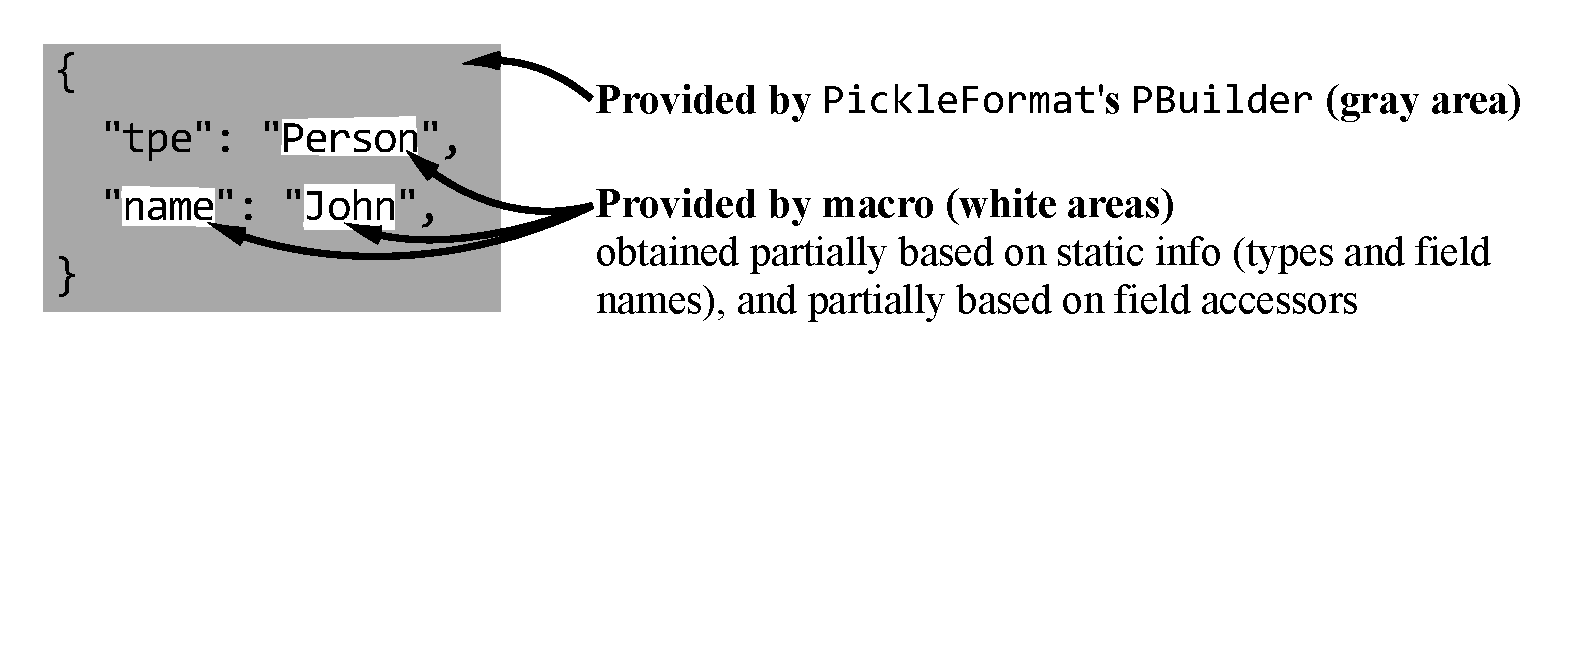
\includegraphics[width=\columnwidth]{generation.pdf}
% \caption{Illustration of pickle template for a sample JSON-formatted pickle.}
% \label{fig:generation}
%\end{figure}

\subsection{Overview}

Our framework generates type-specialized, object-oriented picklers using
compile-time meta programming in the form of {\em macros}. Whenever
a pickler for static type $T$ is required but cannot be found in the implicit
scope, a macro is expanded which generates the required pickler step-by-step
by:

\begin{itemize}
\item Obtaining a type descriptor for the static type of the object to-be-pickled,

\item Building a static {\em intermediate representation} of the object-to-be-pickled,
based on the type descriptor, and

\item Applying a pickler generation algorithm, driven by the static pickler
representation.
\end{itemize}

In our Scala-based implementation, the static type descriptor is generated
automatically by the compiler, and passed as an implicit argument to the
pickle extension method (see Section~\ref{sec:overview}). As a result, such an
implicit \term{TypeTag}\footnotemark[2] does not require changing the invocation in most cases.
(However, it is impossible to generate a \term{TypeTag} automatically if the
type or one of its components is abstract; in this case, an implicit
\term{TypeTag} must be in scope.)

Based on the type descriptor, a static representation, or model, of the
required pickler is built; we refer to this as the {\em Intermediate
Representation} (IR). The IR specifies precisely the set of types for which
our framework can generate picklers automatically. Furthermore, these IRs are composable.

We additionally define a model for composing IRs, which is designed to capture
the essence of Scala's object system as it relates to pickling. The model
defines how the IR for a given type is composed from the IRs of the picklers
of its supertypes. In Scala, the composition of an IR for a class type is
defined based on the linearization of its supertraits. \footnotemark[3]
This model of inheritance is central to the generation framework, and is
formally defined in the following Section \ref{sec:ir}

\subsection{Formal Model of Inheritance}
\label{sec:ir}

The goal of this section is to formally define the representation, or
$IR$, of a static type $T$ as it is used to generate a pickler for
type $T$. We start by defining the syntax of the elements of the IR
(see Def.~\ref{def:elems-ir}).

\begin{defn}{(Elements of IR)}
\label{def:elems-ir}

We define the syntax of values of the IR types.

\begin{align*}
F&        ::= \overline{(f_n, T)}\\
IR&       ::= (T, IR_{opt}, F)\\
IR_{opt}& ::= \epsilon~|~IR
\end{align*}

$F$ represents a sequence of \textit{fields}. We write $\overline{X}$ as
shorthand for sequences, $X_1,\dots,X_n$, and we write tuples
$(X_1,\dots,X_n)$. $f_n$ is a string representing the name of the given field,
and $T$ is its type.

$IR$ represents the pickling information for a class or some other object
type. That is, an $IR$ for type $T$ contains all of the information required
to pickle instances of type $T$, including all necessary static info for
pickling its fields provided by $F$.

$IR_{opt}$ is an optional $IR$; a missing $IR$ is represented using $\epsilon$.
\end{defn}

In our implementation the IR types are represented using case classes. For
example, the following case class represents $IR$s:

\begin{lstlisting}
case class ClassIR(
  tpe: Type,
  parent: ClassIR,
  fields: List[FieldIR]
) extends PickleIR
\end{lstlisting}

Using the definitions of the elements of an IR from Definition \ref{def:elems-ir},
we go on to define a number of useful IR combinators, which form the
basis of our model of inheritance.

% This is the footnote from the definition
\footnotetext[1]{For example, in Scala the linearization is
defined for classes mixing in multiple traits \cite{Odersky2005,ScalaSpec}; in
Java, the linearization function would simply return the chain of
superclasses, not including the implemented interfaces.}


\footnotetext[2]{TypeTags are part of the mainline Scala
compiler since version 2.10. They replace the earlier concept of Manifests,
providing a faithful representation of Scala types at runtime, see Section
\ref{sec:background}.}
\footnotetext[3]{Traits in
Scala can be thought of as a more flexible form of Java-style interfaces that
allow concrete members, and that support a form of multiple inheritance (mix-
in composition) that is guaranteed to be safe based on a linearization order.}

\vspace{0.3cm}

\begin{defn}{(IR Combinators)}

We begin by defining the types of our combinators before we define the
combinators themselves.

\vspace{0.2cm}
{\bf Type Definitions}
{\small
\begin{align*}
\textit{concat}&        : (F, F) \Rightarrow F\\
\textit{extended}&      : (IR, IR) \Rightarrow IR\\
\textit{linearization}& : T \Rightarrow \overline{T}\\
\textit{superIRs}&      : T \Rightarrow \overline{IR}\\
\textit{compose}&       : IR \Rightarrow IR\\
\textit{flatten}&       : IR \Rightarrow IR
\end{align*}
}%

We write function types $X \Rightarrow Y$, indicating a function from type $X$
to type $Y$.

The \textit{linearization} function represents the host language's semantics for the
linearized chain of supertypes.\footnotemark[1]

\vspace{0.3cm}

{\bf Function Definitions}
{\small
\begin{align*}
\textit{concat}(\overline{f}, \overline{g})& = \overline{f}, \overline{g}\\
\textit{extended}(C, D)&                     = (T, C, \textit{fields}(T))\\
                       &                       \qquad \mbox{where}~D = (T, \_, \_)~\land T <: C.1\\
\textit{superIRs}(T)&                        = \lbrack(S, \epsilon, \textit{fields}(S))~|~S\in \textit{linearization}(T)\rbrack\\
\textit{compose}(C)&                         = \textit{reduce}(\textit{superIRs}(C.1),\textit{extended})\\
\textit{flatten}(C)&                         =\left\{ \begin{array}{l}
                                                (C.1, C.2, \textit{concat}(C.3, \textit{flatten(C.2).3})),\\
                                                \qquad\mbox{if}~C.2\neq\epsilon\\
                                                C,~~~\mbox{otherwise}
                                              \end{array} \right.
\end{align*}
}%


The function \textit{concat} takes two sequences as arguments. We
denote concatenation of sequences using a comma. We introduce the
\textit{concat} function for clarity in the definition of \textit{flatten}
(see below); it is simply an alias for sequence concatenation.

\vspace{0.4cm}

\textit{Continued on next page...}

\vspace{0.6cm}

\end{defn}

% \rule{0.9\columnwidth}{0.7pt}

\begin{defn*}{(IR Combinators) -- Continued}

The function \textit{extended} takes two $IR$s, $C$ and $D$, and returns a new
$IR$ for the type of $D$ such that $C$ is registered as its super $IR$.
Basically, \textit{extended} is used to combine a completed $IR$ $C$ with an
incomplete $IR$ $D$ yielding a completed $IR$ for the same type as $D$. When
combining the $IR$s of a type's supertypes, the \textit{extended} function is
used for reducing the linearization sequence yielding a single completed $IR$.

The function \textit{superIRs} takes a type $T$ and returns a sequence of the
IRs of $T$'s supertypes in linearization order.

The function \textit{compose} takes an $IR$ $C$ for a type $C.1$ and returns a
new $IR$ for type $C.1$ which is the composition of the IRs of all supertypes
of $C.1$. The resulting $IR$ is a chain of super IRs according to the
linearization order of $C.1$.

The function \textit{flatten}, given an $IR$ $C$ produces a new $IR$ that
contains a concatenation of all the fields of each nested $IR$. Given
these combinators, the $IR$ of a type $T$ to-be-pickled is obtained
using $IR = flatten(compose((T, \epsilon, \lbrack \rbrack))$.
\end{defn*}

\rule{0.9\columnwidth}{0.7pt}

The above IR combinators have direct Scala implementations in scala/pickling.
For example, function $superIRs$ is implemented as follows:

\begin{lstlisting}
private val f3 = (c: C) =>
  c.tpe.baseClasses
       .map(superSym => c.tpe.baseType(superSym))
       .map(tp => ClassIR(tp, null, fields(tp)))
\end{lstlisting}
\noindent
Here, method \verb|baseClasses| returns the collection of superclass symbols
of type \verb|c.tpe| in linearization order. Method \verb|baseType| converts
each symbol to a type which is, in turn, used to create a \verb|ClassIR|
instance. The semantics of the \verb|fields| method is analogous to the above
$fields$ function.

\subsection{Pickler Generation Algorithm}

The pickler generation is driven by the IR (see Section~\ref{sec:ir}) of a
type to-be-pickled. We describe the generation algorithm in two steps. In the
first step, we explain how to generate a pickler for static type $T$ assuming
that for the dynamic type $S$ of the object to-be-pickled,
\textit{erasure}$(T) =:= S$. In the second step, we explain how to extend the
generation to dynamic picklers which do not require this assumption.

\subsubsection{Pickle Format}
\label{sec:pickleformat}

The pickling logic that we are going to generate contains calls to a pickle
{\em builder} that is used to incrementally construct a pickle. Analogously,
the unpickling logic contains calls to a pickle {\em reader} that is used to
incrementally read a pickle. Importantly, the pickle format that determines
the precise persisted representation of a completed pickle is not fixed.
Instead, the pickle format to be used is selected at compile time-- efficient
binary formats, and JSON are just some examples. This selection is done via
implicit parameters which allows the format to be flexibly selected while
providing a default binary format which is used in case no other format is
imported explicitly.

The pickle format provides an interface which plays the role of a simple,
lower-level ``backend''. Besides a pickle template that is generated inline as
part of the pickling logic, methods provided by pickle builders aim to do as
little as possible to minimize runtime overhead. For example,  the JSON
\term{PickleFormat} included with scala/pickling simply uses an
efficient string builder to concatenate JSON fragments (which are just
strings) in order to assemble a pickle.

The interface provided by \term{PickleFormat} is simple: it basically consists
of two methods (a) for creating an empty builder, and (b) for creating a
reader from a pickle:\footnote{In our actual implementation the
\term{createReader} method takes an additional parameter which is a ``mirror''
used for runtime reflection; it is omitted here for simplicity.}

\begin{lstlisting}
    def createBuilder(): PBuilder
    def createReader(pickle: PickleType): PReader
\end{lstlisting}

The \term{createReader} method takes a pickle of a specific \term{PickleType}
(which is an abstract type member in our implementation); this makes it
possible to ensure that, say, a pickle encapsulating a byte array is not
erroneously attempted to be unpickled using the JSON pickle format. Moreover,
pickle builders returned from \verb|createBuilder| are guaranteed to produce
pickles of the right type.

\begin{lstlisting}
class PBuilder {
  def beginEntry(obj: Any): PBuilder
  def putField(n: String, pfun: PBuilder => Unit): PBuilder
  def endEntry(): Unit
  def result(): Pickle
}
\end{lstlisting}

In the following we're going to show how the \verb|PBuilder| interface is used
by generated picklers; the \verb|PReader| interface is used by generated
unpicklers in an analogous way. The above example summarizes a core
subset of the interface of \verb|PBuilder| that the presented generation
algorithm is going to use.\footnote{It is not necessary that \texttt{PBuilder}
is a class. In fact, in our Scala implementation it is a trait. In Java, it
could be an interface.} The \verb|beginEntry| method is used to indicate the
start of a pickle for the argument obj. The field values of a class instance
are pickled using \verb|putField| which expects both a field name and a lambda
encapsulating the pickling logic for the object that the field points to. The
\verb|endEntry| method indicates the completion of a (partial) pickle of an
object. Finally, invoking \verb|result| returns the completed \verb|Pickle|
instance.

\subsubsection{Tree Generation}

The objective of the generation algorithm is to generate the body of
\term{SPickler}'s \term{pickle} method:

\begin{lstlisting}
  def pickle(obj: T, builder: PBuilder): Unit = ...
\end{lstlisting}

As mentioned previously, the actual pickling logic is synthesized based on the
IR. Importantly, the IR determines which fields are pickled and how. A lot of
the work is already done when building the IR; therefore, the actual tree
generation is rather simple:

\begin{itemize}

\item Emit \verb|builder.beginEntry(obj)|.

\item For each field \term{fld} in the IR, emit \\\verb|builder.putField(${fld.name},b => pbody)|
where \\\verb|${fld.name}| denotes the splicing of \term{fld.name}
into the tree. \term{pbody} is the logic for pickling \term{fld}'s value into
the builder \term{b}, which is an alias of \term{builder}. \term{pbody} is generated
as follows:
  \begin{enumerate}

  \item Emit the field getter logic:
  \\\verb|val v: ${fld.tpe} = obj.${fld.name}|. The
  expression \verb|${fld.tpe}| splices the type of \term{fld} into the generated
  tree; \verb|${fld.name}| splices the name of \term{fld} into the tree.

  \item Recursively generate the pickler for \term{fld}'s type by emitting either
  \\\verb|val fldp = implicitly[DPickler[${fld.tpe}]]| or \verb|val fldp = implicitly[SPickler[${fld.tpe}]]|,
  depending on whether \term{fld}'s type is effectively final or not.

  \item Emit the logic for pickling \term{v} into \term{b}: \verb|fldp.pickle(v, b)|
  \end{enumerate}
\end{itemize}

A practical implementation can easily be refined to support various extensions
of this basic model. For example, support for avoiding pickling fields marked
as {\em transient} is easy with this model of generation-- such fields can
simply be left out of the IR. Or, based on the static types of the picklee and
its fields, we can emit hints to the builder to enable various optimizations.

For example, a field whose type $T$ is {\em effectively final}, \ie it cannot
be extended, can be optimized as follows:

\begin{itemize}
\item Instead of obtaining an implicit pickler of type \term{DPickler[T]}, it is
sufficient to obtain an implicit pickler of type \term{SPickler[T]}, which is
more efficient, since it does not require a dynamic dispatch step like
\term{DPickler[T]}

\item The field's type does not have to be pickled, since it can be reconstructed
from its owner's type.
% \footnote{Our implementation makes heavy use of this
% optimization for pickling collections of primitives efficiently; see
% Section~\ref{sec:optimize}.}
\end{itemize}

Pickler generation is compositional; for example, the generated pickler for a
class type with a string-typed field re-uses the string pickler. This is
achieved by generating picklers for parts of an object type using invocations
of the form \verb|implicitly[DPickler[T]]|. This means that if there is
already an implicit value of type \term{DPickler[T]} in scope, it is used for
pickling the corresponding value. Since the lookup and binding of these
implicit picklers is left to a mechanism outside of pickler generation, what's
actually generated is a {\em pickler combinator} which returns a {\em pickler}
composed of {\em existing picklers} for parts of the object to-be-pickled.
More precisely, pickler generation provides the following composability
property:

\begin{prop}{(Composability)}
A generated pickler \term{p} is composed of implicit picklers of the required
types that are in scope at the point in the program where \term{p} is
generated.
\end{prop}

Since the picklers that are in scope at the point where a pickler is generated
are under programmer control, it is possible to import manually written
picklers which are transparently picked up by the generated pickler. Our
approach thus has the attractive property that it is an ``open-world''
approach, in which it is easy to add new custom picklers for selected types at
exactly the desired places while integrating cleanly with generated picklers.

\subsubsection{Dispatch Generation}

So far, we have explained the generation of the pickling logic of static
picklers. Dynamic picklers require an additional dispatch step to make sure
subtypes of the static type to-be-pickled are pickled properly. The generation
of a \term{DPickler[T]} is triggered by invoking
\verb|implicitly[DPickler[T]]| which tries to find an implicit of type
\term{DPickler[T]} in the current implicit scope. Either there is already an
implicit value of the right type in scope, or the only matching implicit is an
implicit def provided by the pickling framework which generates a
\term{DPickler[T]} on-the-fly. The generated dispatch logic has the following
shape:

\begin{lstlisting}
    val clazz = if (picklee != null) picklee.getClass else null
    val pickler = clazz match {
      case null => implicitly[SPickler[NullTpe]]
      case c1 if c1 == classOf[S1] => implicitly[SPickler[S1]]
      ...
      case cn if cn == classOf[Sn] => implicitly[SPickler[Sn]]
      case _ => genPickler(clazz)
    }
\end{lstlisting}

The types $S1, \dots, Sn$ are known subtypes of the picklee's type $T$. If $T$
is a sealed class or trait with final subclasses, this set of types is always
known at compile time. However, in the presence of separate compilation it is,
generally, possible that a picklee has an unknown runtime type; therefore, we
include a default case (the last case in the pattern match) which dispatches
to a runtime pickler that inspects the picklee using (runtime) reflection.

If the static type $T$ to be pickled is annotated using the
\term{$@$pickleable} annotation, all subclasses are guaranteed to extend the
predefined \verb|HasPickler| interface trait. Consequently, a more optimal
dispatch can be generated in this case:

\begin{lstlisting}
    val pickler =
      if (picklee != null) {
        val hasp = picklee.asInstanceOf[HasPickler]
        hasp.getPickler.asInstanceOf[SPickler[T]]
      }
      else implicitly[SPickler[NullTpe]]
\end{lstlisting}

\subsection{Runtime Picklers}
\label{sec:runtime-pickler}

One goal of our framework is to generate as much pickling code at compile time
as possible. However, due to the interplay of subclassing with both separate
compilation and generics, we provide a runtime fall back capability to handle
the cases that cannot be resolved at compile time.

{\bf Subclassing and separate compilation}: A situation arises where it's
impossible to statically know all possible subclasses. In this case there are
three options: (1) provide a custom pickler, and (2) use an annotation which
is described in Section \ref{sec:pickleable-annotation}. In the case where
neither a custom pickler nor an annotation is provided, our framework can
inspect the instance to-be-pickled at runtime to obtain the pickling logic.
This comes with some runtime overhead, but in Section \ref{sec:evaluation} we
present results which suggest that this overhead is not necessary in many
cases.

For the generation of runtime picklers our framework supports two possible
strategies:

\begin{itemize}
\item Runtime interpretation of a type-specialized pickler
\item Runtime compilation of a type-specialized pickler
\end{itemize}

\paragraph{Interpreted runtime picklers.} If the runtime type of an object is
unknown at compile time, e.g., if its static type is \term{Any}, it is
necessary to carry out the pickling based on inspecting the type of the object
to-be-pickled at runtime. We call picklers operating in this mode ``interpreted
runtime picklers'' to emphasize the fact that the pickling code is not
partially evaluated in this case. An interpreted pickler is created based on
the runtime class of the picklee. From that runtime class it is possible to
obtain a runtime type descriptor.

\begin{itemize}
\item to build a static intermediate representation of the type (which describes all its fields with their types, etc.)
\item to determine in which way the picklee should be pickled (as a primitive or not).
\end{itemize}

In case the picklee is of primitive type, there are no fields to be pickled.
Otherwise, the value and runtime type of each field is obtained, so that it
can be written to the pickle.

%\todo We mention in the bulleted list above runtime compilation but don't explain it


\begin{figure*}[ht!]
 \centering
 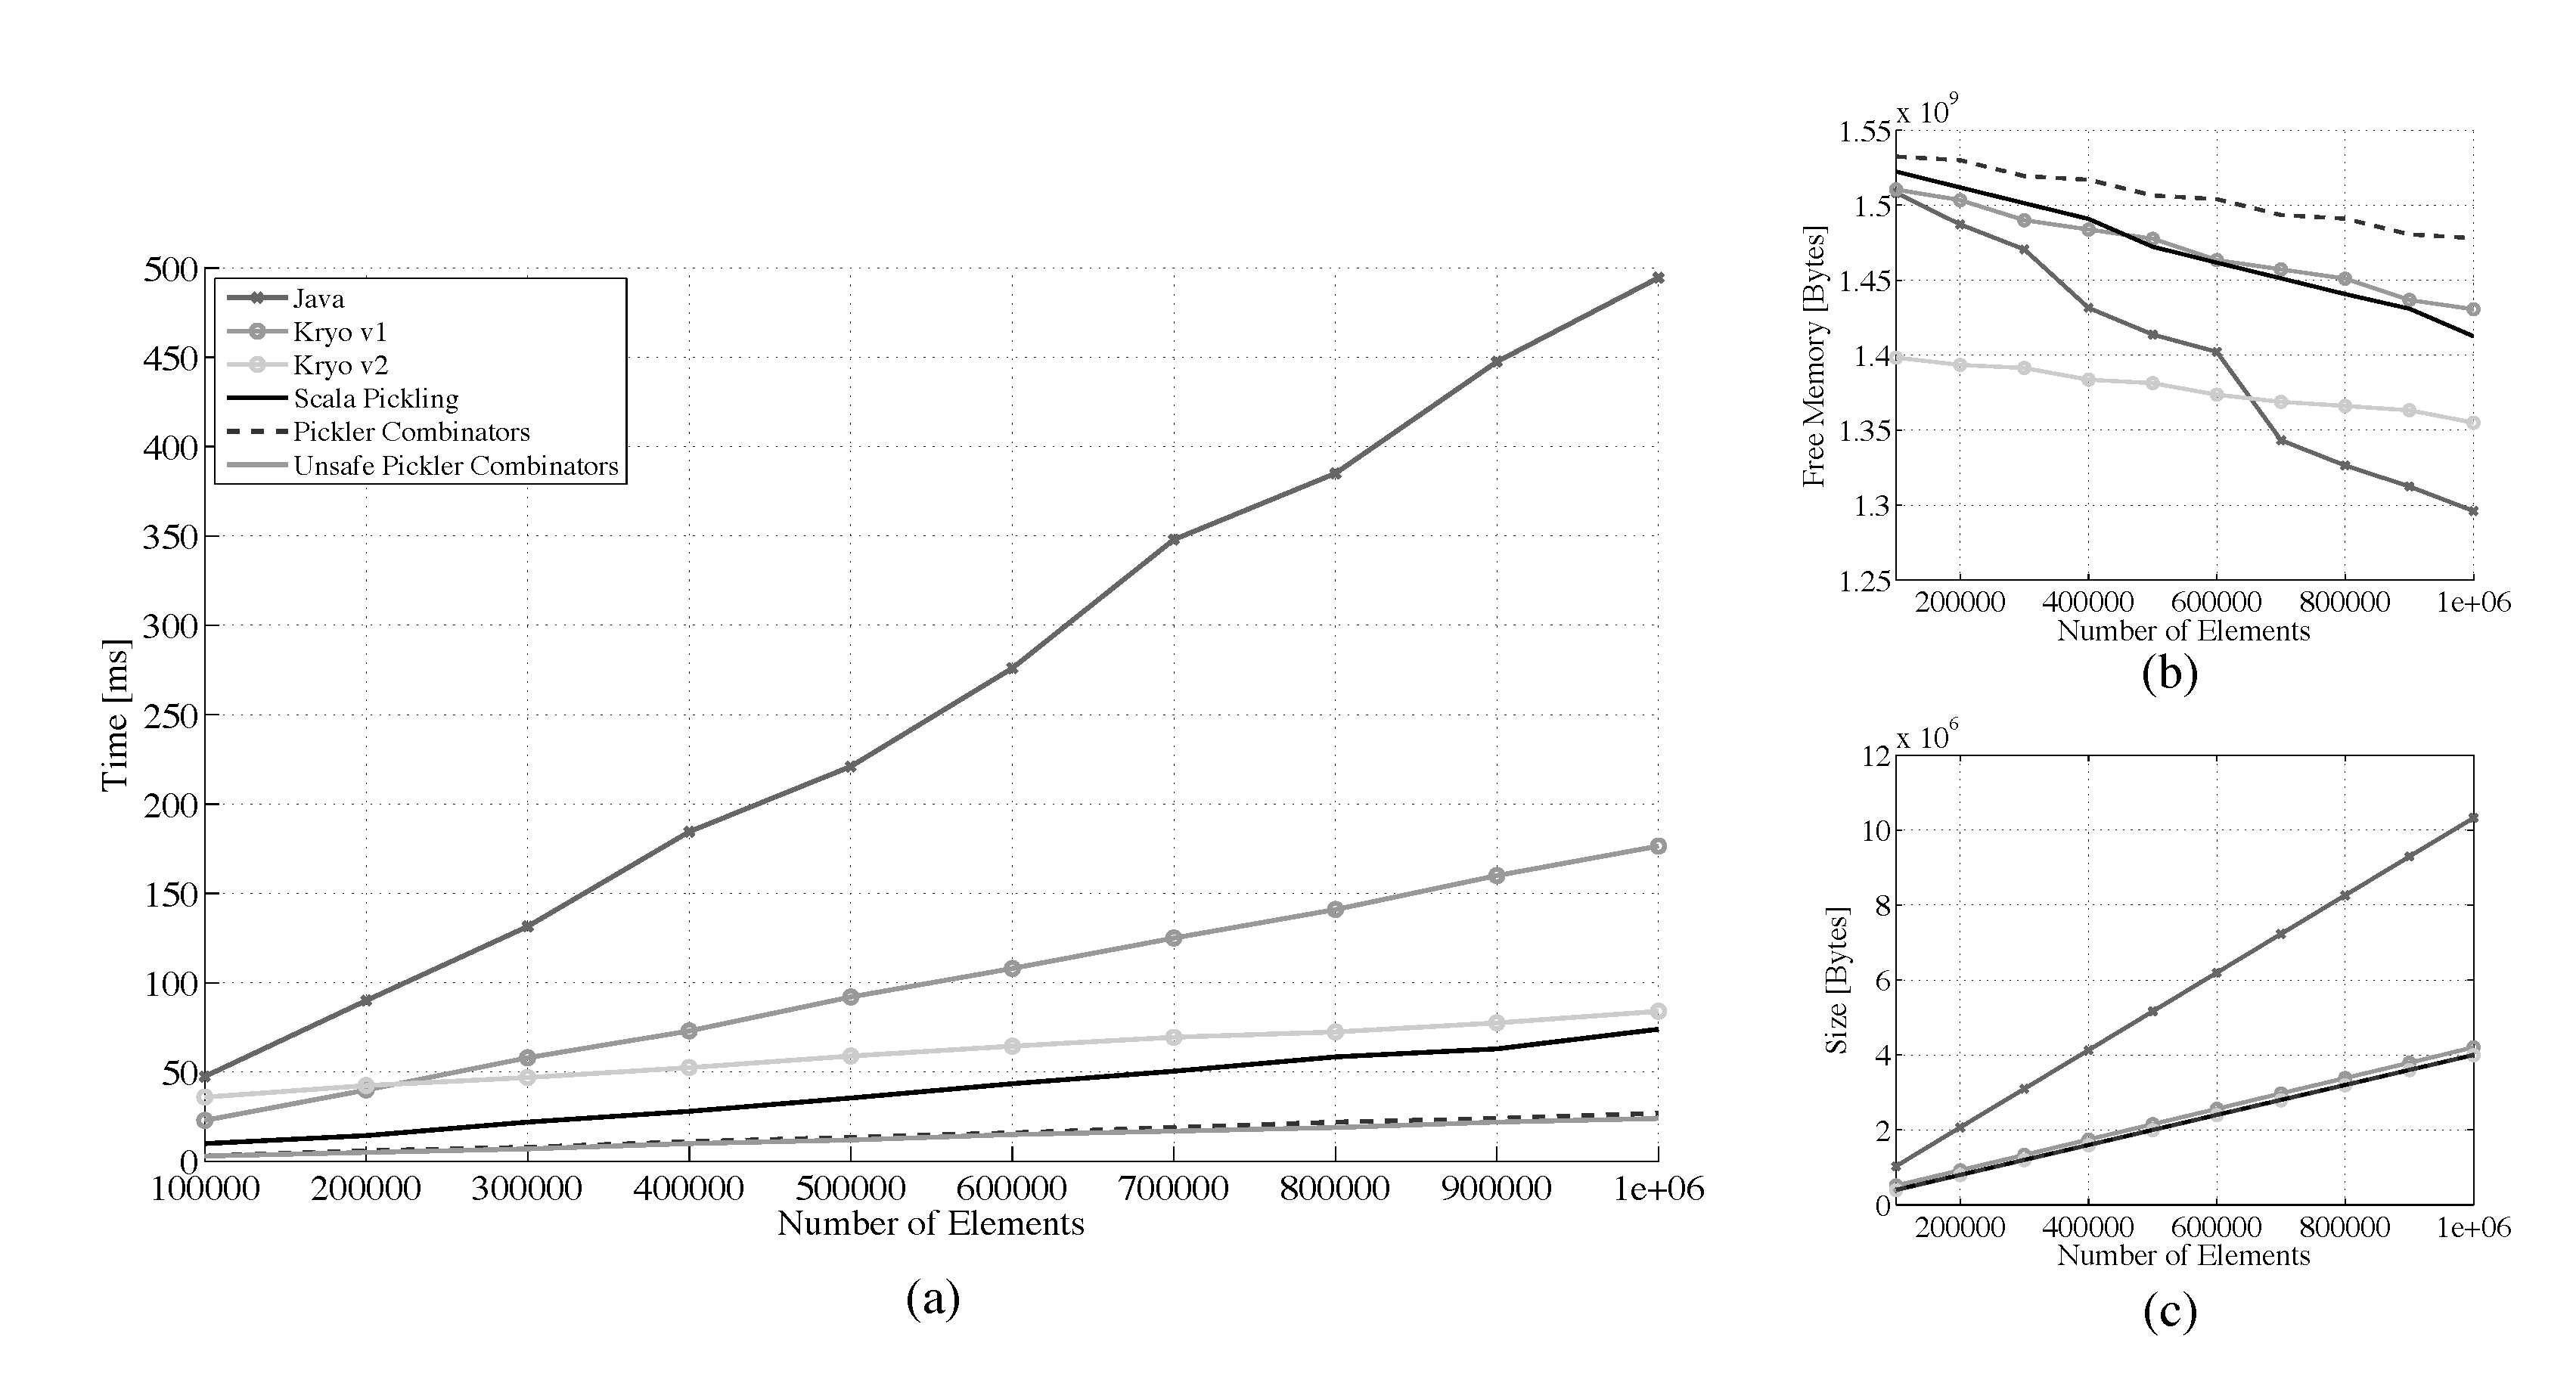
\includegraphics[width=\textwidth]{travInt-all.pdf}
 \caption{Results for pickling and unpickling an immutable
   \texttt{Vector[Int]} using different frameworks.}
 \label{fig:results-vector}
\end{figure*}

\subsection{Generics and Arrays}

\paragraph{Subclassing and generics.} The combination of subclassing and generics
poses a similar problem to that introduced above in Section \ref{sec:runtime-pickler}.
For example, consider a generic class \term{C},

\begin{lstlisting}
    class C[T](val fld: T) { ... }
\end{lstlisting}

A \term{Pickler[C[T]]} will not be able to pickle the field \term{fld} if its
static type is unknown. To support pickling instances of generic classes, our
framework falls back to using runtime picklers for pickling fields of generic
type. So, when we have access to the runtime type of field \term{fld}, we can
either look up an already-generated pickler for that runtime type, or we can
generate a suitable pickler dynamically.

\paragraph{Arrays.} Scala arrays are mapped to Java arrays;  the two have the
same runtime representation. However, there is one important difference: Java
arrays are covariant whereas Scala arrays are invariant. In particular, it is
possible to pass arrays from Java code to Scala code. Thus, a class \verb|C|
with a field \verb|f| of type \verb|Array[T]| may have an instance at runtime
that stores an \verb|Array[S]| in field \verb|f| where \verb|S| is a subtype
of \verb|T|. Pickling followed by unpickling must instantiate an
\verb|Array[S]|. Just like with other fields of non-final reference type, this
situation requires writing the dynamic (array) type name to the pickle. This
is possible, since array types are not erased on the JVM (unlike generic
types). This allows instantiating an array with the expected dynamic type upon
unpickling. At the time of writing only support for primitive arrays has been
implemented in scala/pickling.


\subsection{Object Identity and Sharing}
\label{sec:object-identity}

Object identity enables the existence of complex object graphs, which
themselves are a cornerstone of object-oriented programming. While in
Section~\ref{sec:data-types-in-distributed-applications} we show that pickling
\textit{flat} object graphs is most common in big data applications, a general
pickling framework for use with an object-oriented language must not only
support flat object graphs, it must also support cyclic object graphs.

Supporting such cyclic object graphs in most object-oriented languages,
however, typically requires sophisticated runtime support, which is known to
incur a significant performance hit. This is due to the fact that pickling
graphs with cycles requires tracking object identities at runtime, so that
pickling terminates and unpickling can faithfully reconstruct the graph
structure.

To avoid the overhead of tracking object identities unanimously for all
objects, ``runtime-based'' serialization frameworks like Java or Kryo have to
employ reflective/introspective checks to detect whether identities are
relevant.\footnote{With Kryo, some of this overhead can be avoided when using custom, handwritten serializers.}

Scala/pickling, on the other hand, employs a hybrid compile-time/runtime
approach. This makes it possible to avoid the overhead of object identity
tracking in cases where it is statically known to be safe, which we show in
Section~\ref{sec:data-types-in-distributed-applications} is typically
important in big data applications.

The following Section~\ref{sec:object-tracking} outlines how object identity
is tracked in scala/pickling. It also explains how the management of object
identities enables a {\em sharing} optimization. This sharing optimization is
especially important for persistent data structures, which are commonly used
in Scala. Section~\ref{sec:object-graph-analysis} explains how compile-time
analysis is used to reduce the amount of runtime checking in cases where
object graphs are statically known to be acyclic.

\subsubsection{Object Tracking}
\label{sec:object-tracking}

During pickling, a pickler keeps track of all objects that are part of the
(top-level) object to-be-pickled in a table. Whenever an object that's part of
the object graph is pickled, a hash code based on the identity of the object
is computed. The pickler then looks up whether that object has already been
pickled, in which case the table contains a unique integer ID as the entry's
value. If the table does not contain an entry for the object, a unique ID is
generated and inserted, and the object is pickled as usual. Otherwise, instead
of pickling the object again, a special \verb|Ref| object containing the integer ID
is written to the pickle.\footnote{Several strategies exist to avoid preventing pickled objects from being garbage collected. Currently, for each top-level object to-be-pickled, a new hash table is created.}
During unpickling, the above process is reversed by maintaining a
mapping\footnote{This can be made very efficient by using a map implementation which is more efficient for integer-valued keys, such as a resizable array.}
from integer IDs to unpickled heap objects.

This approach to dealing with object identities also enables sharing, an
optimization which in some big data applications can improve system throughput
by reducing pickle size. Scala's immutable collections hierarchy is one
example of a set of data structures which are persistent, which means they
make use of sharing. That is, object subgraphs which occur in multiple
instances of a data structure can be shared which is more efficient than
maintaining multiple copies of those subgraphs

Scala/pickling's management of object identities benefits instances of such
data structures as follows. First, it reduces the size of the computed pickle,
since instead of pickling the same object instance many times, compact
references (\verb|Ref| objects) are pickled. Second, pickling time also has
the potential to be reduced, since shared objects have to be pickled only
once.

\subsubsection{Static Object Graph Analysis}
\label{sec:object-graph-analysis}

When generating a pickler for a given type \verb|T|, the IR is analyzed to
determine whether the graph of objects of type \verb|T| may contain cycles.
Both \verb|T| and the types of \verb|T|'s fields are examined using a breadth-
first traversal. Certain types are immediately excluded from the traversal,
since they cannot be part of a cycle. Examples are primitive types, like
\verb|Double|, as well as certain immutable reference types that are final,
like \verb|String|. However, the static inspection of the IR additionally
allows Scala-pickling to traverse sealed class hierarchies.

For example, consider this small class hierarchy:

\begin{lstlisting}
final class Position(p: Person, title: String)
sealed class Person(name: String, age: Int)
final class Firefighter(name: String, age: Int, salary: Int)
  extends Person(name, age)
final class Teacher(name: String, age: Int, subject: String)
  extends Person(name, age)
\end{lstlisting}

In this case, upon generating the pickler for class \verb|Position|, it is
detected that no cycles are possible in the object graphs of instances of type
\verb|Position|. While \verb|Position|'s \verb|p| field has a reference type,
it cannot induce cycles, since \verb|Person| is a sealed class that has only
final subclasses; furthermore, \verb|Person| and its subclasses have only
fields of primitive type.

In addition to this analysis, our framework allows users to disable all
identity tracking programmatically, in case it is known that the graphs of
(all) pickled objects are acyclic. While this switch can boost performance, it
also disables opportunities for sharing (see above), and may thus lead to
larger ``pickles''.



\section{Implementation}

The presented framework has been fully implemented in Scala.
The object-oriented pickler combinators presented in
Section~\ref{sec:oopicklers}, including their implicit selection and
composition, can be implemented using stable versions of the standard, open-source
Scala distribution. The extension of our basic model with
automatic pickler generation has been implemented using the experimental
macros feature introduced in Scala 2.10.0. Macros can be thought of as a
more regularly strucutred, localized, and more stable alternative to compiler
plugins. To simplify tree generation, our implementation leverages a
quasiquoting library for Scala's macros~\cite{Quasiquotes}.



%\subsection{Optimizations}
%\label{sec:optimize}

%\section{Temporary TODOs}

%\subsection{Recursive Types}

%\todo what to do with this?

%Recursive types are used in many common data structures like lists, trees etc. Here we show how recursive types are supported in our framework.

%Example (we show a non-generic class hierarchy for simplicity):

%\begin{lstlisting}
%    abstract class IntTree
%    class Empty extends IntTree
%    class Fork(left: IntTree, elem: Int, right: IntTree)
%\end{lstlisting}

\begin{figure*}[ht!]
 \centering
 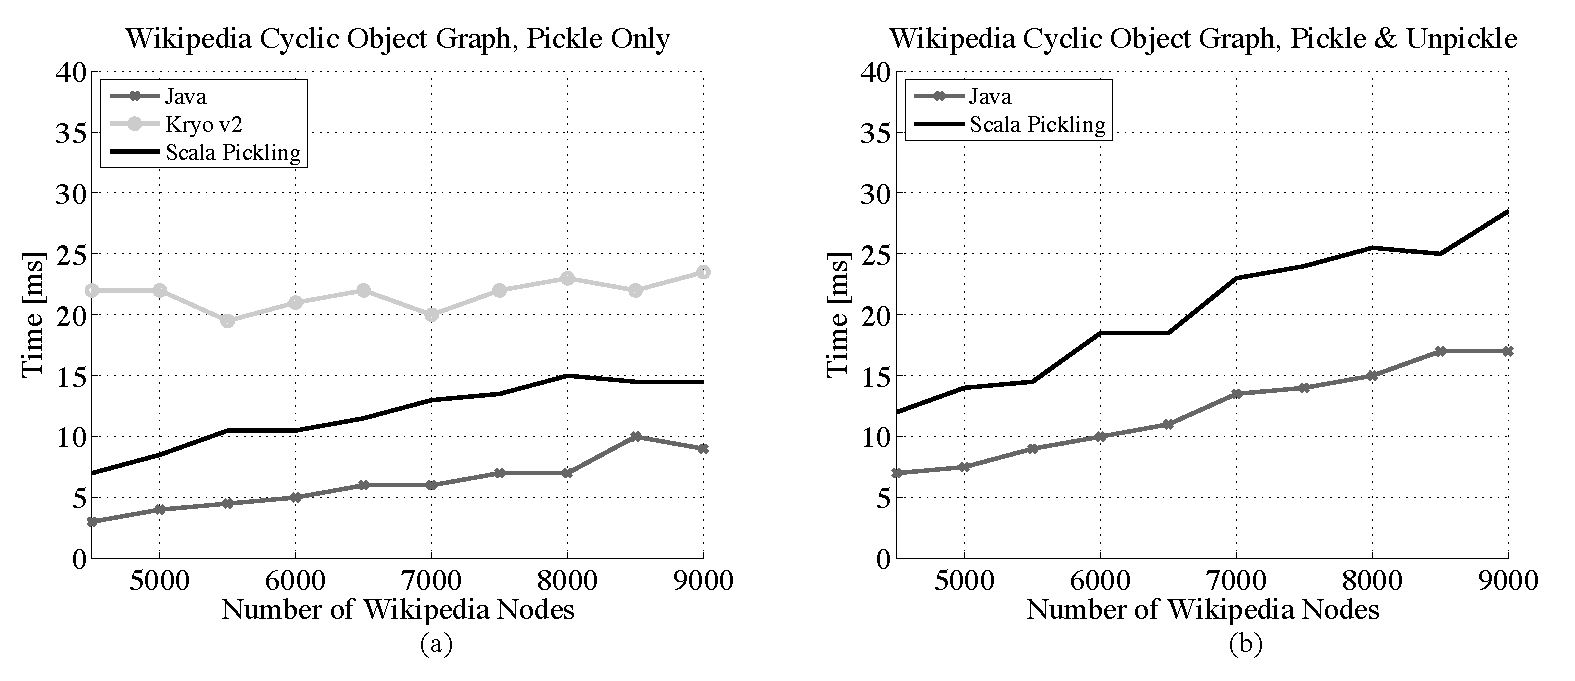
\includegraphics[width=\textwidth]{wikigraph.pdf}
 \caption{}
 \label{fig:wikigraph}
\end{figure*}

\section{Experimental Evaluation}
\label{sec:evaluation}

In this section we present first results of an experimental evaluation
of our pickling framework. Our goals are
\begin{enumerate}
\item to evaluate the performance of automatically-generated picklers
  compared to manually written picklers, analyzing the memory usage
  compared to other serialization frameworks,
\item to provide a survey of the properties of data types that are
  commonly used in distributed computing frameworks and applications.
\end{enumerate}\noindent
In the process we are going to evaluate the performance of our
framework alongside two popular and industrially-prominent serialization frameworks
for the JVM, Java's native serialization and Kryo.\footnote{We select Kryo and Java because, like scala/pickling, they both are ``automatic''. That is, they require no schema or extra compilation phases, as is the case for other frameworks such as Apache Avro and Google Protobuf.}

\subsection{Experimental Setup}

The following benchmarks were run on a MacBook Pro with a 2.7 GHz
Intel Core i7 processor with 16 GB of memory running Mac OS X version
10.8.2 and Oracle's Java HotSpot(TM) 64-Bit Server VM version
1.6.0\_43. In all cases we used the following configuration flags:
\texttt{-Xms1536M -Xmx4096M -Xss2M -XX:MaxPermSize=512M -XX:+UseParallelGC}. Each benchmark was run on a warmed-up JVM. The result shown is the median of 9 such ``warm'' runs.

\begin{figure}[ht!]
 \centering
 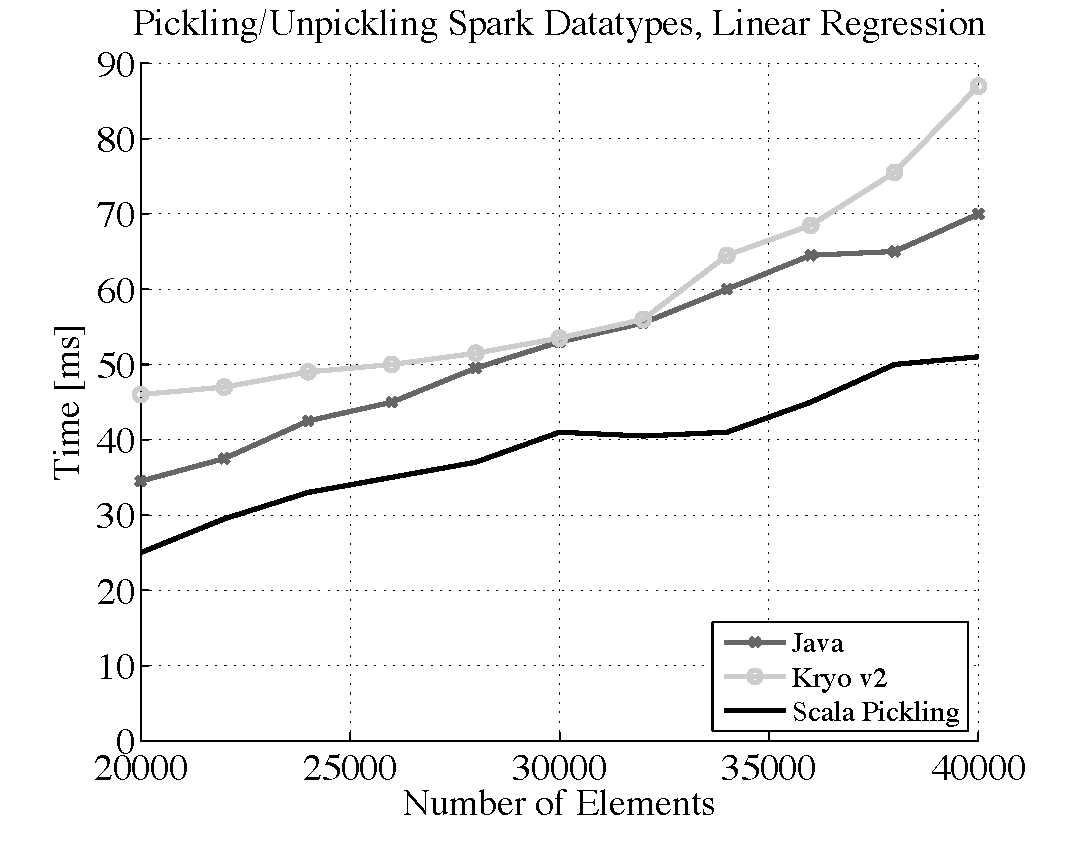
\includegraphics[width=\columnwidth]{sparklr.pdf}
 \caption{Results for pickling and unpickling an immutable
   \texttt{Vector[Int]} using different frameworks.}
 \label{fig:spark}
\end{figure}

\subsection{Microbenchmark: Collections}

In the first microbenchmark we evaluate the performance of our
framework when pickling standard collection types. We compare against
three other serialization frameworks: Java's native serialization,
Kryo, and a combinator library of naive handwritten pickler combinators. All
benchmarks are compiled and run using Scala version 2.9.3, except for
the present framework which depends on an experimental macro system,
as well as a couple of minor bug fixes that exist only in a current
development version of Scala.

The benchmark logic is very simple: an immutable collection of type
\verb|Vector[Int]| is created which is first pickled (or serialized)
to a byte array, and then unpickled. While \verb|List| is the protypical collection type used in Scala, we ultimately chose \verb|Vector| as
Scala's standard \verb|List| type could not be serialized out-of-the-box\footnote{We register each class with Kryo, an optional step that improves performance.}
using Kryo, because it is a recursive type in Scala. In order to use Scala's standard List type with Kryo, one must write a custom serializer, which would sidestep the objective of this benchmark, which is to compare the speed of {\em generated} picklers.

The results are
shown in Figure~\ref{fig:results-vector} (a). As can be seen, Java is markedly slower than any other framework. This is likely due to the expensive runtime cost of the JVM's calculation of the runtime transitive closure of the objects to be serialized. For 1,000,000 elements, Java finishes in 491ms while scala/pickling finishes in 86ms, or a factor 5.7 faster. As can be seen, the
performance of our prototype is faster than Kryo for small to moderate-sized collections, and is on par with Kryo or even slightly slower for large collections. For a Vector with 100,000 elements, Kryo finishes in 36ms while scala/pickling finishes in 10ms-- a factor of 3.6 in favor of scala/pickling. Conversely, for a Vector of 1,000,000 elements, Kryo finishes in 82ms whereas scala/pickling finishes in 86ms. The
performance of manually written pickler combinators, however, is still
considerably better. This is likely due to the fact that pickler combinators require no runtime checks whatsoever-- picklers combinators are defined per type, and manually composed, requiring no such check. In principle, it should be possible to generate code
that is as fast as these pickler combinators in the case
where static picklers can be generated\footnote{As a framework intended for eventual production use, we are actively seeking to bring performance closer to that of fully-static hand-composed pickler combinators. Towards that aim, we maintain a full benchmark suite at \url{http://lampwww.epfl.ch/~hmiller/pickling}}.

Figure~\ref{fig:results-vector} (b) shows the corresponding memory usage; on the
y-axis the value of \texttt{System.freeMemory} is shown. This plot
reveals evidence of a key property of Kryo, namely (a) that its memory usage
is quite high compared to other frameworks, and (b) that its
serialization is stateful because of internal buffering. In fact, when
preparing these benchmarks we had to manually adjust Kryo buffer sizes
several times to avoid buffer overflows. It turns out the main reason
for this is that Kryo reuses buffers whenever possible when
serializing one object after the other. In many cases the
newly pickled object is simply append at the current position in the
existing buffer which results in unexpected buffer growth. Our
framework does not do any buffering which makes its behavior very
predictable, but does not necessarily maximize its performance.

Finally, Figure~\ref{fig:results-vector} (c) shows the relative sizes of the serialized data. For a Vector of 1,000,000 elements, Java required 10,322,966 bytes. As can be seen, all other frameworks perform on par with another, requiring about 40\% of the size of Java's binary format. Or, in order of largest to smallest; Kryo v1 - 4,201,152 bytes; Kryo v2 - 4,088,570 bytes; scala/pickling 4,000,031 bytes; and Pickler Combinators 4,000,004 bytes.

\subsection{Data Types in Distributed Frameworks and Applications}
\label{sec:data-types-in-distributed-applications}

\begin{figure*}[ht!]
 \centering
 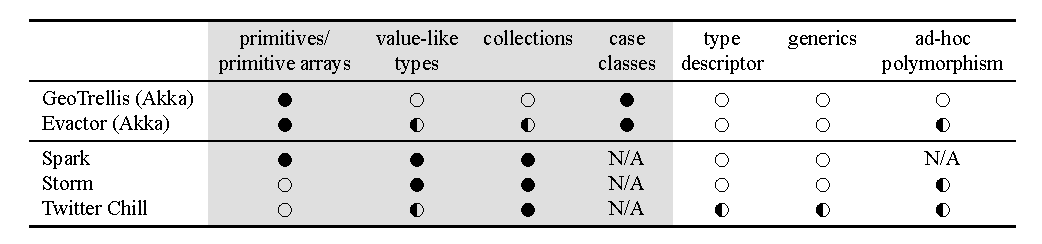
\includegraphics[width=0.9\textwidth]{application-table.pdf}
 \vspace{-1em}
 \caption{Scala types used in industrial distributed frameworks and applications.}
 \label{fig:application-table}
\end{figure*}

% \begin{table*}
% \centering
% \begin{tabular}{l c c c c c c c}
% \toprule % Top horizontal line
% & primitives/ & value-like & collections & case & type & generics & subtyping \\ % Column names row
% & primitive arrays & types &  & classes & descriptor &  & polymorphism \\ % Column names row
% \midrule % In-table horizontal line
% GeoTrellis (Akka) & $\CIRCLE$ & $\Circle$     & $\Circle$     & $\CIRCLE$ & $\Circle$     & $\Circle$     & $\Circle$ \\
% Evactor (Akka)    & $\CIRCLE$ & $\LEFTcircle$ & $\LEFTcircle$ & $\CIRCLE$ & $\Circle$     & $\Circle$     & $\LEFTcircle$ \\
% \midrule % In-table horizontal line
% Spark             & $\CIRCLE$ & $\CIRCLE$     & $\CIRCLE$     & $\LEFTcircle$ & $\Circle$     & $\Circle$     & $\Circle$ \\
% Storm             & $\Circle$ & $\CIRCLE$     & $\CIRCLE$     & N/A       & $\Circle$     & $\Circle$     & $\LEFTcircle$ \\
% Twitter Chill     & $\Circle$ & $\LEFTcircle$ & $\CIRCLE$     & $\LEFTcircle$ & $\LEFTcircle$ & $\LEFTcircle$ & $\LEFTcircle$ \\
% \bottomrule % Bottom horizontal line
% \end{tabular}\vspace{0.5em}
% \mbox{\centering{\bf Legend:}~~~~$\CIRCLE$: Heavy Use~~~~$\LEFTcircle$: Light Use~~~~$\Circle$: No Use}
% % \caption{Table caption text} % Table caption, can be commented out if no caption is required
% % \label{tab:template} % A label for referencing this table elsewhere, references are used in text as \ref{label}
% \end{table*}

Figure~\ref{fig:application-table} shows a summary of the most
important data types used in popular distributed computing frameworks
like Spark~\cite{Zaharia2012} and Storm~\cite{Storm}.
The fully shaded circles in the table representing ``heavy use'' means either
(a) a feature is used frequently in application-level data types or
(b) a feature is used frequently in data types that the framework registers
(with its underlying serialization system.
Half-shaded circles in the table representing ``light use'' mean a feature is used
only infrequently in the data types used in applications or registered by
frameworks. We categorize the data types shown in this table into two groups.

In the first group at the top are distributed \emph{applications}
using data types suitable for distributed event processing and message
passing. We consider two representative open-source applications:
GeoTrellis~\cite{GeoTrellis} is a geographic data
processing engine for high performance applications used by the US
federal government among others.  Evactor is a complex event processor
based on actors. Both applications use Akka~\cite{Akka}, an
event-driven middleware for distributed message passing. However, the
properties of the exchanged messages are markedly different. Messages
in GeoTrellis typically contain large amounts of geographic raster
data, stored in arrays of primitives. Messages in Evactor represent
individual events which typically contain only a few values of
primitive types. Both applications make use of Scala's case classes
which are most commonly used as message types in actor-based
applications.

The second group in the bottom half of Figure~\ref{fig:application-table}
consists of distributed computing {frameworks}. What this table
suggests is that the majority of distributed computing frameworks and
applications requires pickling collections of various
types. Interestingly, application-level data types tend to use arrays
with primitive element type; a sign that there is a great need to
provide easier ways to process ``big data'' efficiently. From the
table it is also clear that case classes tend to be primarily of
interest to application code whereas frameworks like Spark tend to
prefer the use of simple collections of primitive type
internally. What's more, the demand for pickling generics seems to be
lower than the need to support subtyping polymorphism (our framework
supports both, though). At least in one case (Twitter's Chill~\cite{TwitterChill}) a
framework explicitly serializes Manifests, type descriptors for Scala
types, which are superceded by TypeTags (see
Section~\ref{sec:reflection})
The shaded area (which groups ``heavily-used'' features across
applications/frameworks) shows that collections are often used in distributed
code, in particular with primitive element types. This motivates the choice of
our collections micro benchmark.




\section{Other Related Work}
\label{sec:related-work}

Pickling in programming languages has a long history dating back to
CLU~\cite{HerlihyL82} and Modula-3~\cite{CardelliDJKN89}. The most
closely-related contemporary work is in two areas. First, pickling in
object-oriented languages, for example, in Java (see the Java Object
Serialization Specification~\cite{JavaSerialization}), in .NET, and in
Python~\cite{Rossum07}; second, work on pickler combinators in
functional languages which we have already discussed in the
introduction. The main difference of our framework compared to
pickling, or serialization, in widespread OO languages is that our
approach does not require special support by the underlying
runtime. In fact, the core concepts of object-oriented picklers as
presented in this paper can be realized in most OO languages with
generics.

While work on pickling is typically focused on finding optimally compact
representations for data \cite{EveryBitCounts}, not all work has focused only
on distribution and persistence of ground values. Pickling has also been
used to distribute and persist code to implement module systems~\cite{Roy99,Rossberg2007}.
There is a body of work on maximizing sharing of runtime data
structures~\cite{appel93hashconsing,Elsman2005,TackKS06} which we believe
could be applied to the pickler combinators presented in
Section~\ref{sec:oopicklers}; however, a complete solution is beyond the scope
of the present paper.


% \section{Future Work}

\section{Conclusion and Future Work}

We have introduced a model of pickler combinators which supports core
concepts of object-oriented programming including subtyping polymorphism
with open class hierarchies. Furthermore, we have shown how this model
can be augmented by a composable mechanism for static pickler
generation which is effective in reducing boilerplate and in ensuring
efficient pickling. Thanks to a design akin to an object-oriented
variation of type classes known from functional programming, the
presented framework enables retrofitting existing types and
third-party libraries with pickling support. Experiments suggest that
static generation of pickler combinators can outperform
state-of-the-art serialization frameworks and significantly reduce
memory usage.

In future work we plan to further optimize the pickler generation and
to extend the framework with support for closures.

% A reference to Table \ref{tab:template}.


% \appendix
% \section{Appendix Title}

% This is the text of the appendix, if you need one.

% \acks

% Acknowledgments, if needed.

% We recommend abbrvnat bibliography style.


% The bibliography should be embedded for final submission.

%\begin{thebibliography}{}
%\softraggedright

%\bibitem[Smith et~al.(2009)Smith, Jones]{smith02}
%P. Q. Smith, and X. Y. Jones. ...reference text...

%\end{thebibliography}

\begin{spacing}{0.9}
\bibliographystyle{abbrvnat}
\bibliography{bib}
\end{spacing}

\end{document}
